%!TEX root = Manuscript.tex

\chapter{Precise matching}
\label{chap:Precisematching}
\minitoc

\section{Introduction}
\subsection{Motivation and objective}
%Inter-epoch image pairs are roughly aligned 
The rough co-registration stage elaborated in Section~\ref{chap:RoughCoReg} laid a solid foundation for matching inter-epoch images, as it roughly aligned images from different epochs in a globally consistent way. However, the alignment is not accurate enough for high precision cartography. 
Therefore, we propose a precise matching stage to get matches with higher accuracy, which benefits from the guidance of rough co-registration to guarantee both robustness and precision. 
For each inter-epoch image pair $I^{e_1}$ and $I^{e_2}$ to be matched, our goal is to find precise matches $M({\mathbf{K}^{e_1},\mathbf{K}^{e_2}})$ ($\mathbf{K}^{e_i}$ represents keypoints extracted in image $I^{e_i}$). 
Based on the roughly co-registered orientations and \ac{DSM}s resulted from Chapter~\ref{chap:RoughCoReg}, 
we can readily predict a potential matching point $\widetilde{\mathbf{K}}^{e_2}$ in $I^{e_2}$ for keypoint $\mathbf{K}^{e_1}$. % in $I^{e_1}$. 
As rough co-registration provides robust yet imprecise alignment, the precise matching point for keypoint $\mathbf{K}^{e_1}$ should not be far away from the predicted point $\widetilde{\mathbf{K}}^{e_2}$. Therefore, we can narrow down the search space in precise matching stage by only considering the local neighborhood of the predicted point $\widetilde{\mathbf{K}}^{e_2}$ to reduce ambiguity tremendously. 
%Similar to rough co-registration, both SIFT and SuperGlue are adopted in our precise matching pipeline.\\
For hand-crafted methods like SIFT, the strategy of predicting keypoints followed by narrowing down the search space can be readily applied. Besides, as SIFT provides explicitly the scale and rotation angle of the keypoints, we can take advantage of that and introduce an idea of \textit{SclRotCheck}, which is to check if the scale and rotation of the keypoints coincide with the scale and rotation predicted by rough co-registration.\\
For learned methods like SuperGlue, it is not easy to modify the algorithm, as it inevitably involves retraining the model, which is not easy due to lack of training data. Therefore we propose an \textit{one-to-one tiling scheme} (not to confuse with the \textit{one-to-many tiling scheme} presented in Section \ref{chap:RoughCoReg}) to feed roughly aligned patches into the model to reduce ambiguity. Its merits are twofold: (1) up-scaling the learning based feature matching algorithms to high resolution imagery, as directly feeding the original images often lead to inaccurate results; (2) narrowing down the searching space in an elegant way without modifying the model.
%key-point predictions from one can be readily made 
%\subsection{Motivation}
\subsection{Contributions}
%Under guidance of rough co-registration, we 
%We reduce the 
\zll{Our contribution is to combine rough co-registration results, \textit{one-to-one tiling scheme}, \textit{SclRotCheck} and 3D-RANSAC into a reliable pipeline to recover both robust and precise matches, more specifically, we:\\}
%\zll{Our main contribution is integrating the following points into establishing a pipeline for rough co-registration between inter-epoch image pairs:\\}

%to recover robust and accurate matches by drastically reducing ambiguity under guidance of rough co-registration, improving matching performance with \textit{one-to-one tiling scheme} and \textit{SclRotCheck}, and employing 3D information to reject false matches. More precisely, our main contributions include:\\
\begin{enumerate}
	\item reduce the difficulty in precise matching under the guidance of co-registered orientations and \ac{DSM}s by narrowing down the search space.
	\item introduce \textit{one-to-one tiling scheme} to (1) scale-up the deep learning methods and (2) reduce matching ambiguity without retraining the model.
	\item introduce \textit{SclRotCheck} to remove potential matches whose scale ratio and rotation difference are not consistent with the prediction of rough co-registration.
	\item perform RANSAC to estimate the 3D Helmert transformation between surfaces (i.e., \ac{DSM}s) calculated in different epochs. Compared to the classical essential/fundamental matrix filtering, with less data (3 versus 5 points) we impose stricter rules (1D versus 2D constraint). %on the sets of points. 
	%\item \zll{integrate cross correlation to }
\end{enumerate}

\section{Methodology}
To compute precise {inter-epoch} matches, we perform matching on original RGB images {under the guidance of co-registered orientations and \ac{DSM}s}. {It consists of extracting tentative inter-epoch matches, followed by a 3D-RANSAC filter and a cross correlation stage to remove outliers.} The workflow is displayed in Figure~\ref{WorkflowPatch}(a).
\par
%We choose matching RGB images for precise matching instead of \ac{DSM}s, as the \ac{DSM}s are noisy due to (1) low radiometric quality of historical images and (2) errors inevitably introduced during calculated \ac{DSM}s. In Section ~\ref{CompareRGBDSM} %Appendix~\ref{chap:appendix4} 
We choose matching RGB images for precise matching instead of \ac{DSM}s, as \ac{DSM}s are (1) noisy due to errors inevitably introduced during calculating \ac{DSM}s and (2) monotonous in flat terrain due to lack of textures. In Section ~\ref{CompareRGBDSM} we displayed the matching results on both RGB images and \ac{DSM}s over the same area. It demonstrates that more matches are found in \ac{DSM}s but the accuracy is inferior. As our goal is to recover accurate matches, the RGB images are more suitable than \ac{DSM}s. Besides, it is more efficient as calculating high resolution \ac{DSM}s is computationally demanding.\\

\begin{figure*}[htbp]
	\begin{center}
		\subfigure[Workflow]{
			\begin{minipage}[t]{1\linewidth}
				\centering
				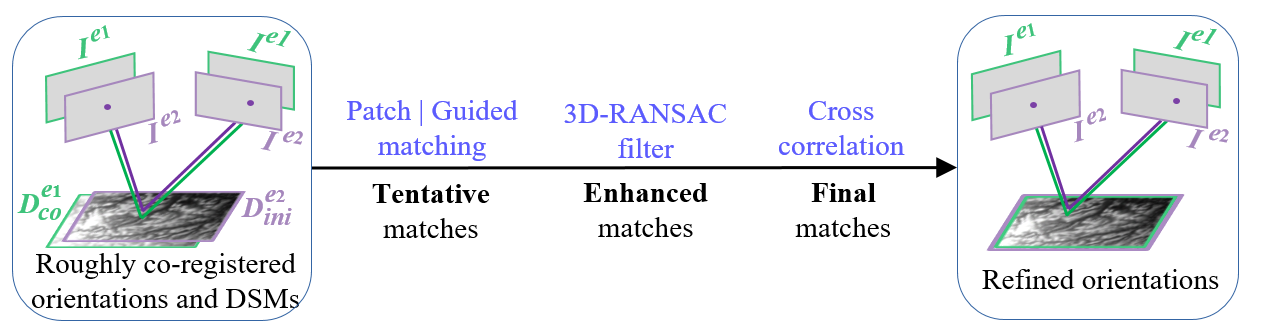
\includegraphics[width=1\columnwidth]{images/Chapitre4/precisematching.png}
			\end{minipage}%
		}
		\subfigure[Patch matching]{
			\begin{minipage}[t]{0.35\linewidth}
				\centering
				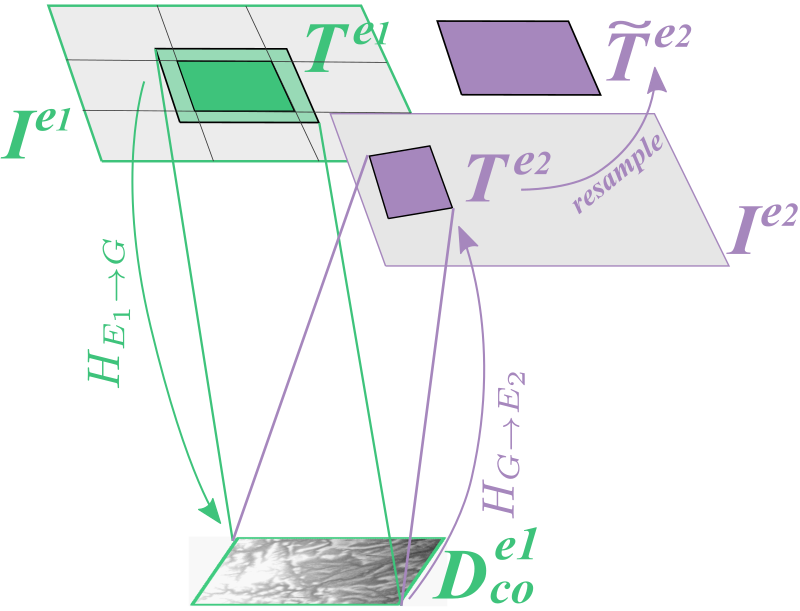
\includegraphics[width=4.5cm]{images/Chapitre4/patchmatching.png}
			\end{minipage}%
		}
		\subfigure[Buffer zone of tiles]{
			\begin{minipage}[t]{0.25\linewidth}
				\centering
				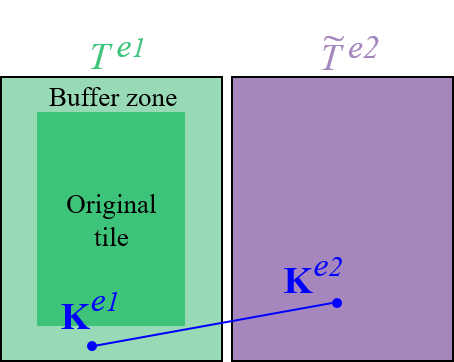
\includegraphics[width=3.8cm]{images/Chapitre4/tilingScheme.png}
			\end{minipage}%
		}
		\subfigure[Guided matching]{
			\begin{minipage}[t]{0.35\linewidth}
				\centering
				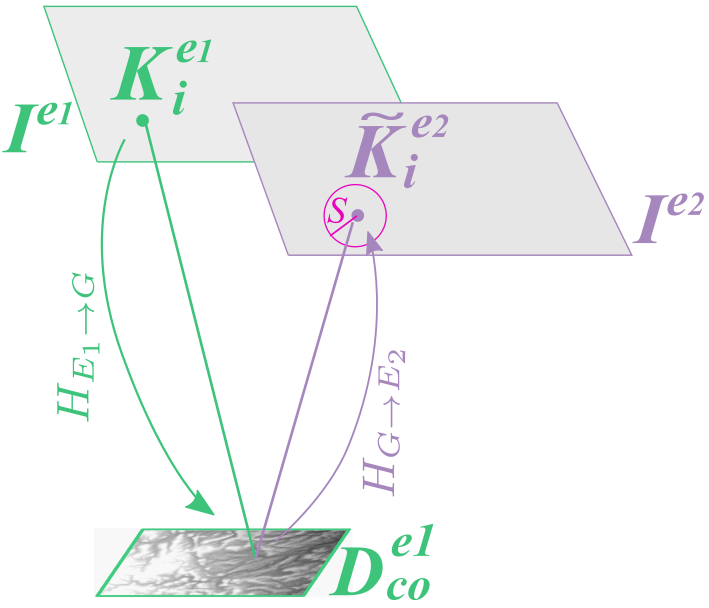
\includegraphics[width=4.5cm]{images/Chapitre4/guidedmatching.png}
			\end{minipage}%
		}
		\caption{(a) Workflow of precise matching. It is carried out by performing patch or guided matching to obtain tentative matches, followed by 3D-RANSAC filter and cross correlation, giving rise to final matches. (b) and (d) illustrate toy-examples of the patch and guided matching, respectively. (c) displays the match where $\mathbf{K}^{e_1}$ exceeds the original tile size (dark green area) and is therefore abandoned.}
		\label{WorkflowPatch}
	\end{center}
\end{figure*}

\subsection{Get tentative matches with patch/guided matching}\label{patch matching}
We offer two alternatives to recover tentative matches: patch or guided matching. \zll{The former uses learned features, while the latter uses hand-crafted features.} %{The former has better overall} performance while the latter is more efficient in terms of the use of memory and CPU resources.\\
Patch matching often gives larger number of matches, while guided matching is in general more efficient.
%\subsubsection{Patch matching for learned features}
\paragraph{Patch matching for learned features.}
\zll{For patch matching, we propose a \textit{one-to-one tiling scheme} to improve matching performance of learned features and reduce ambiguity at the same time. It is illustrated in Figure~\ref{WorkflowPatch}(b), and elaborated below:\\
%{{It} is based on \textit{one-to-one tiling scheme}}, as shown in Figure~\ref{WorkflowPatch}(b). Besides, an example of patch matching applied on an image pair is displayed in Figure~\ref{patchexample} for better understanding. It works as follows:
\begin{enumerate}
	%\item Crop the master RGB image $I^{e_1}$ into M tiles ($T^{e_1}$) of certain size (640$\times$480 pixels in our experiments), with a buffer zone (64 pixels in the width and 48 pixels in the height in our experiments) overlapped with each other;
	\item Crop the master RGB image $I^{e_1}$ into M original tiles of size $SZ_{one-to-one}^{Orig}$, and expand them with a buffer zone of size $SZ_{buffer}$ (as shown in Figure~\ref{WorkflowPatch}(c)), giving rise to M buffered tiles ($T^{e_1}$) of size $SZ_{one-to-one}$;
	\item Project each buffered tile $T^{e_1}$ onto the \ac{DSM} $D_{co}^{e_1}$ and backproject to secondary RGB image $I^{e_2}$ to find the corresponding tile $T^{e_2}$;
	\item Resample $T^{e_2}$ to $\widetilde{T}^{e_2}$, so that the tile pair $P({T^{e_1},\widetilde{T}^{e_2}})$ is free from differences of rotation, scale and extent;
\end{enumerate}
We apply SuperGlue on each tile pair $P({T^{e_1},\widetilde{T}^{e_2}})$ to find matches $M({\mathbf{K}^{e_1},\mathbf{K}^{e_2}})$ ($\mathbf{K}^{e_i}$ represents keypoints in image $I^{e_i}$), and merge the matches together by removing the ones with $\mathbf{K}^{e_1}$ located in the buffer zone. 
%\begin{enumerate}
%	\item Apply SuperGlue on tile pair $P({T^{e_1},\widetilde{T}^{e_2}})$ to find matches $M({\mathbf{K}^{e_1},\mathbf{K}^{e_2}})$ ($\mathbf{K}^{e_i}$ represents keypoints in $I^{e_i}$);
%	\item Merge together the matches from M tile pairs by removing the matches with $\mathbf{K}^{e_i}$ located in the buffer zone.\\
%\end{enumerate}
As the orientations and \ac{DSM}s are only roughly co-registered, we take into account the margin of error when projecting tiles to overlapping images. This is why we add a buffer zone in the tile $T^{e_1}$.\\ %In our experiments, the sizes of original and buffered tiles are set to 512$\times$384 and 640$\times$480 pixels individually.\\
For better understanding, in Figure~\ref{patchexample} we display an example of an inter-epoch image pair, as well as the tile pairs resulted from the \textit{one-to-one tiling scheme}.\\}
Our patch matching experiments are performed based on SuperGlue, however, other learned methods can be adopted readily. \\

\begin{figure*}[htbp]
	\begin{center}
		\subfigure[Example of an image pair]{
			\begin{minipage}[t]{1\linewidth}
				\centering
				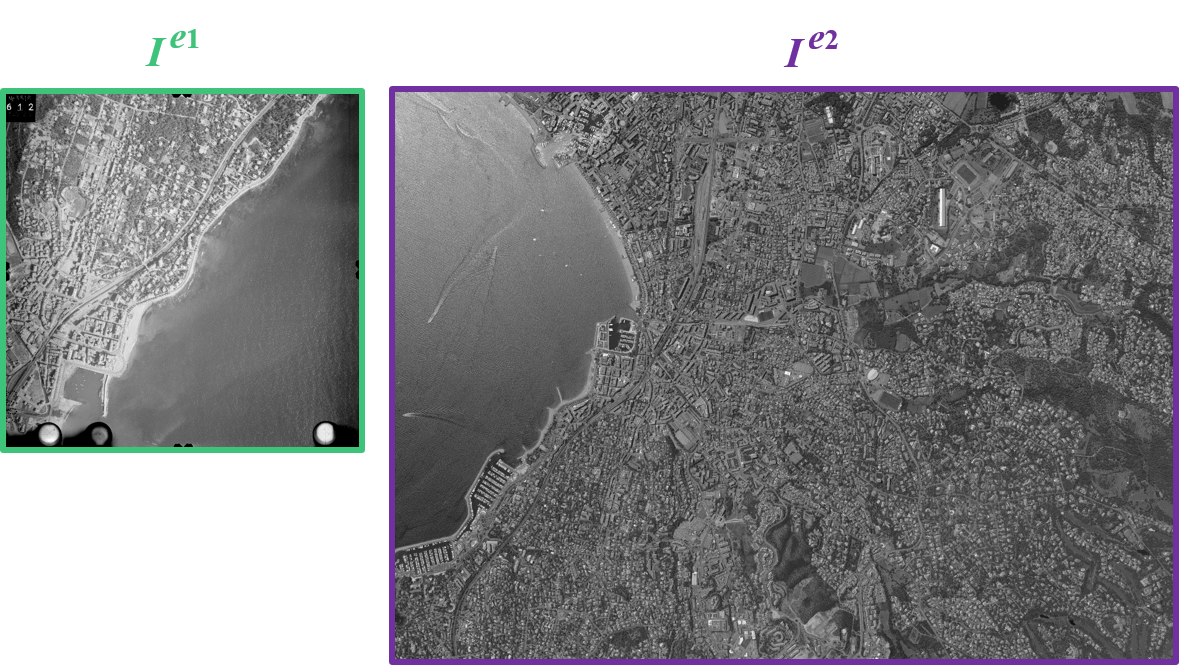
\includegraphics[width=1\columnwidth]{images/Chapitre4/example.png}
			\end{minipage}%
		}
		\subfigure[Demonstration of tile pairs]{
			\begin{minipage}[t]{1\linewidth}
				\centering
				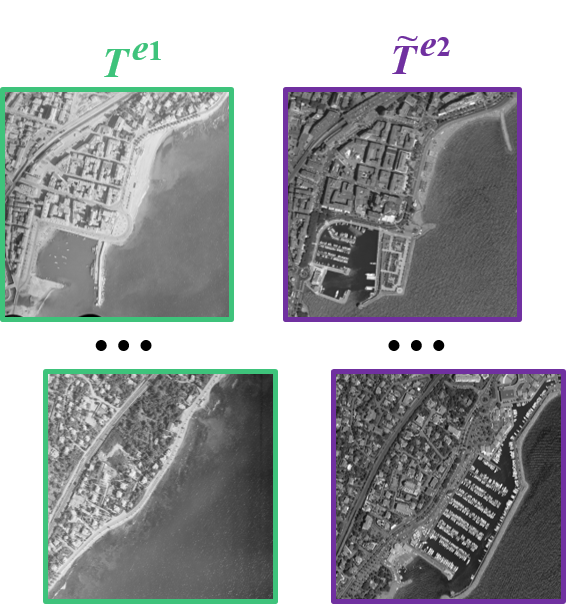
\includegraphics[width=1\columnwidth,trim=10 0 0 0,clip]{images/Chapitre4/patchexample.png}
			\end{minipage}%
		}
		%			\subfigure[Example of keypoint prediction]{
		%		\begin{minipage}[t]{1\linewidth}
		%			\centering
		%			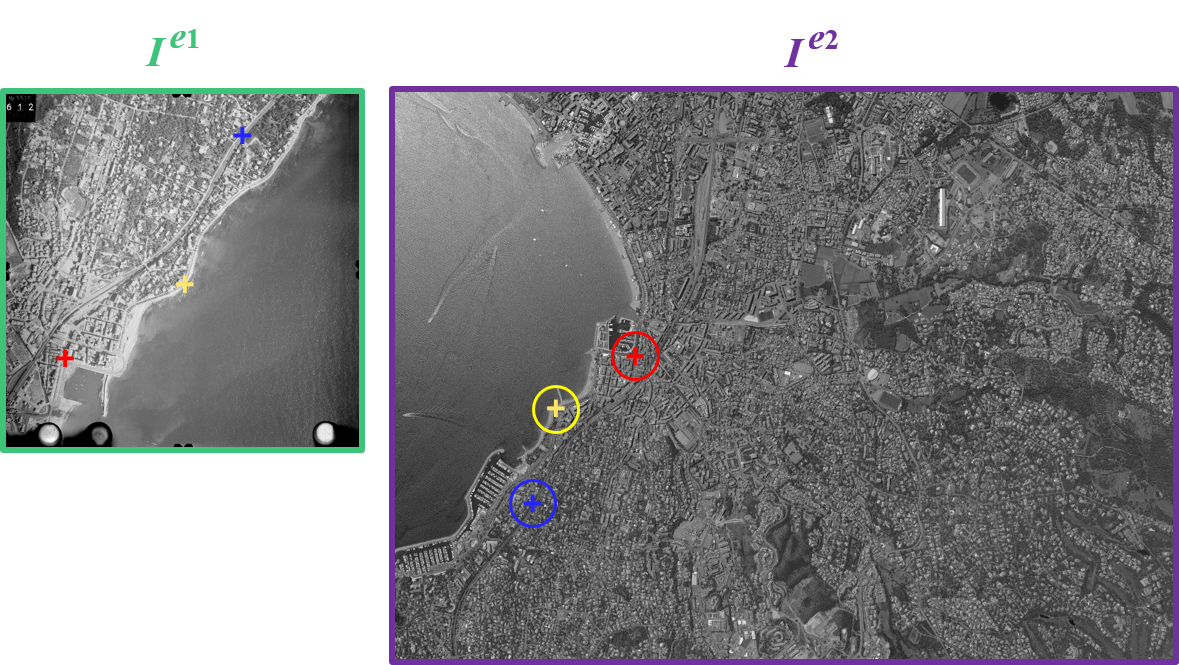
\includegraphics[width=1\columnwidth]{images/Chapitre4/guidedexample.png}
		%		\end{minipage}%
		%	}
		\caption{Illustration of patch matching applied on an inter-epoch image pair. (a) The master image ($I^{e_1}$) and secondary image ($I^{e_2}$) are taken at Fr{\'e}jus in 1954 and 2014 individually. (b) Tile pairs resulted from \textit{one-to-one tiling scheme}, the tile zones before and after buffering are marked as red and green rectangles.}
		\label{patchexample}
	\end{center}
\end{figure*}

\begin{figure*}[htbp]
	\begin{center}
		%\subfigure[Example of keypoint prediction]{
		%	\begin{minipage}[t]{1\linewidth}
				\centering
				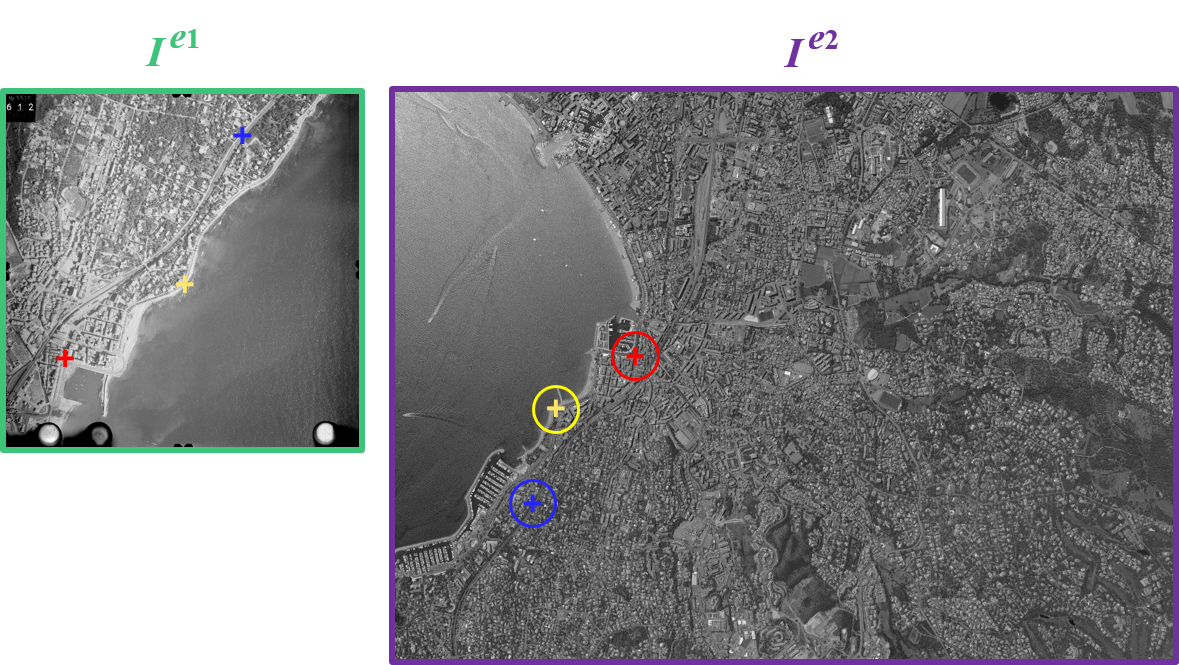
\includegraphics[width=1\columnwidth]{images/Chapitre4/guidedexample.png}
		%	\end{minipage}%
		%}
		\caption{Illustration of keypoint prediction (cross symbols) accompanied with search space (circles), the master image ($I^{e_1}$) and secondary image ($I^{e_2}$) are taken at Fr{\'e}jus in 1954 and 2014 individually.}
		\label{guidedexample}
	\end{center}
\end{figure*}

%\subsubsection{Guided matching for hand-crafted features} 
\paragraph{Guided matching for hand-crafted features.} 
The patch matching substitute orientated towards hand-crafted features is the guided matching, as shown in Figure~\ref{WorkflowPatch}(d). It leverages the positions of predicted keypoints, {the known scale ratio and rotation differences to narrow down the list of the matching candidates}. In our experiments, we use the SIFT points, but the pipeline is suitable to any hand-crafted extractor. 
%Illustration of guided matching applied on an image pair is displayed in Figure~\ref{patchexample} for better understanding. 
%The strategy {is as follows}:\\
It consists of the following steps:\\
\begin{enumerate}
	\item {Compute the scale ratio $R_{scl}$ and the rotation $D_{rot}$ between two images by sequentially projecting the $I^{e_1}$ image corners to the co-registered \ac{DSM} $D_{co}^{e_1}$ and to image $I^{e_2}$;} %\textcolor{red}{Project the image corners of $I^{e_1}$ to the co-registered \ac{DSM} $D_{co}^{e_1}$, and back-project them to $I^{e_2}$ to estimate the scale ratio $R_{scl}$ and angle difference $D_{ang}$ between images $I^{e_1}$ and $I^{e_2}$.}
	\item Extract keypoints $\mathbf{K}^{e_1}$ in image $I^{e_1}$ and $\mathbf{K}^{e_2}$ in image $I^{e_2}$;
	\item Intersect the keypoints $\mathbf{K}^{e_1}$ with the co-registered \ac{DSM} $D_{co}^{e_1}$;
	\item Back-project them to image $I^{e_2}$, giving rise to predicted keypoints $\widetilde{\mathbf{K}}^{e_2}$;
	\item Search for a subset of points in $\mathbf{K}^{e_2}$ located within a radius $S$ centered at the predicted positions $\widetilde{\mathbf{K}}^{e_2}$;%\textcolor{green}{(I don't use a distance threshold.)}
	\item Remove candidate matches whose scales and rotations computed by SIFT are incoherent with $R_{scl}$ and $D_{rot}$;% computed from image orientations and the co-registered \ac{DSM} (i.e., step 1);
	\item {Find the best matches with mutual nearest neighbor combined with the first to second nearest neighbor ratio test~\cite{lowe2004distinctive}.}
\end{enumerate}
For better understanding, in Figure~\ref{guidedexample} we display an example of an inter-epoch image pair, with keypoint prediction (cross symbols) accompanied with search space (circles) superposed on them.\\

\subsection{Get enhanced matches with 3D-RANSAC}
To compute enhanced matches, we apply a 3D-RANSAC filter on the previously obtained tentative matches. {More precisely, we do the following}: (1) for each match $M({\mathbf{K}^{e_1},\mathbf{K}^{e_2}})$, the keypoints $\mathbf{K}^{e_1}$ and $\mathbf{K}^{e_2}$ are projected onto \ac{DSM} $D_{co}^{e_1}$ and $D_{ini}^{e_2}$ individually to get 3D matching points $M({\mathbf{KG}^{e_1},\mathbf{KG}^{e_2}})$; and (2) {the matches} $M({\mathbf{KG}^{e_1},\mathbf{KG}^{e_2}})$ are iteratively sampled to compute the 3D Helmert transformation RANSAC model:
\begin{equation}
\left [ \begin{array}{c}
{KG}_x^{e_2}\\
{KG}_y^{e_2}\\
{KG}_z^{e_2}
\end{array}
\right ] =\lambda \cdot \mathbf{R} \cdot {\left [ \begin{array}{c}
	{KG}_x^{e_1}\\
	{KG}_y^{e_1}\\
	{KG}_z^{e_1}
	\end{array}
	\right ]} + \left [ \begin{array}{c}
\Delta_x\\
\Delta_y\\
\Delta_z
\end{array}
\right ]. \label{eq:3DSimP}
\end{equation}
where $\lambda$ is the scale factor, $\mathbf{R}$ is the rotation matrix and $\left [ \begin{array}{c}
\Delta_x, \Delta_y, \Delta_z
\end{array}
\right ]$ $^{^T}$ is the translation vector.
\zll{Matches within $T_r$ of its predicted position (i.e., $\lvert \mathbf{KG}^{e_2} - (\lambda \cdot \mathbf{R} \cdot \mathbf{KG}^{e_1} + \Delta) \rvert < T_r$) are considered as inliers.}
%We set the number of RANSAC iterations to 1000, and consider matches within $T_r$ of its predicted position as inliers. In our experiment, {$T_r$ was set to 10$\times$$GSD$ where $GSD$ is the mean ground sampling distance in the coordinate frame of epoch ${e_2}$. This distance is computed as the ground distance between two adjacent image pixels.}

\subsection{Get final matches with cross correlation}
In the preceding step we got rid of a substantial number of outliers, however, we believe that not all outliers could be identified. 
Besides, our goal is to get a moderate number of reliable matches instead of many unreliable ones. Therefore we introduce a different filtering method (i.e., cross correlation) to further remove false matches. \zll{Even though cross correlation itself is not discriminative and efficient enough when used alone, it fits well in our pipeline as we already recovered many discriminative and well-distributed matches before applying it.} 
%another filtering method, cross-correlation, which is different than the previous step to remove false matches slipped through the net. 
Matches with their correlation scores below a predefined threshold $T_c$ are discarded. The correlation window size was set to be large enough to take into account the context around a point (32$\times$32 pixels in our experiment). Figure~\ref{crossc} shows an example of a false match (red) eliminated by cross correlation, while the true match (blue) is kept.\\
\begin{figure*}[htbp]
	\begin{center}
		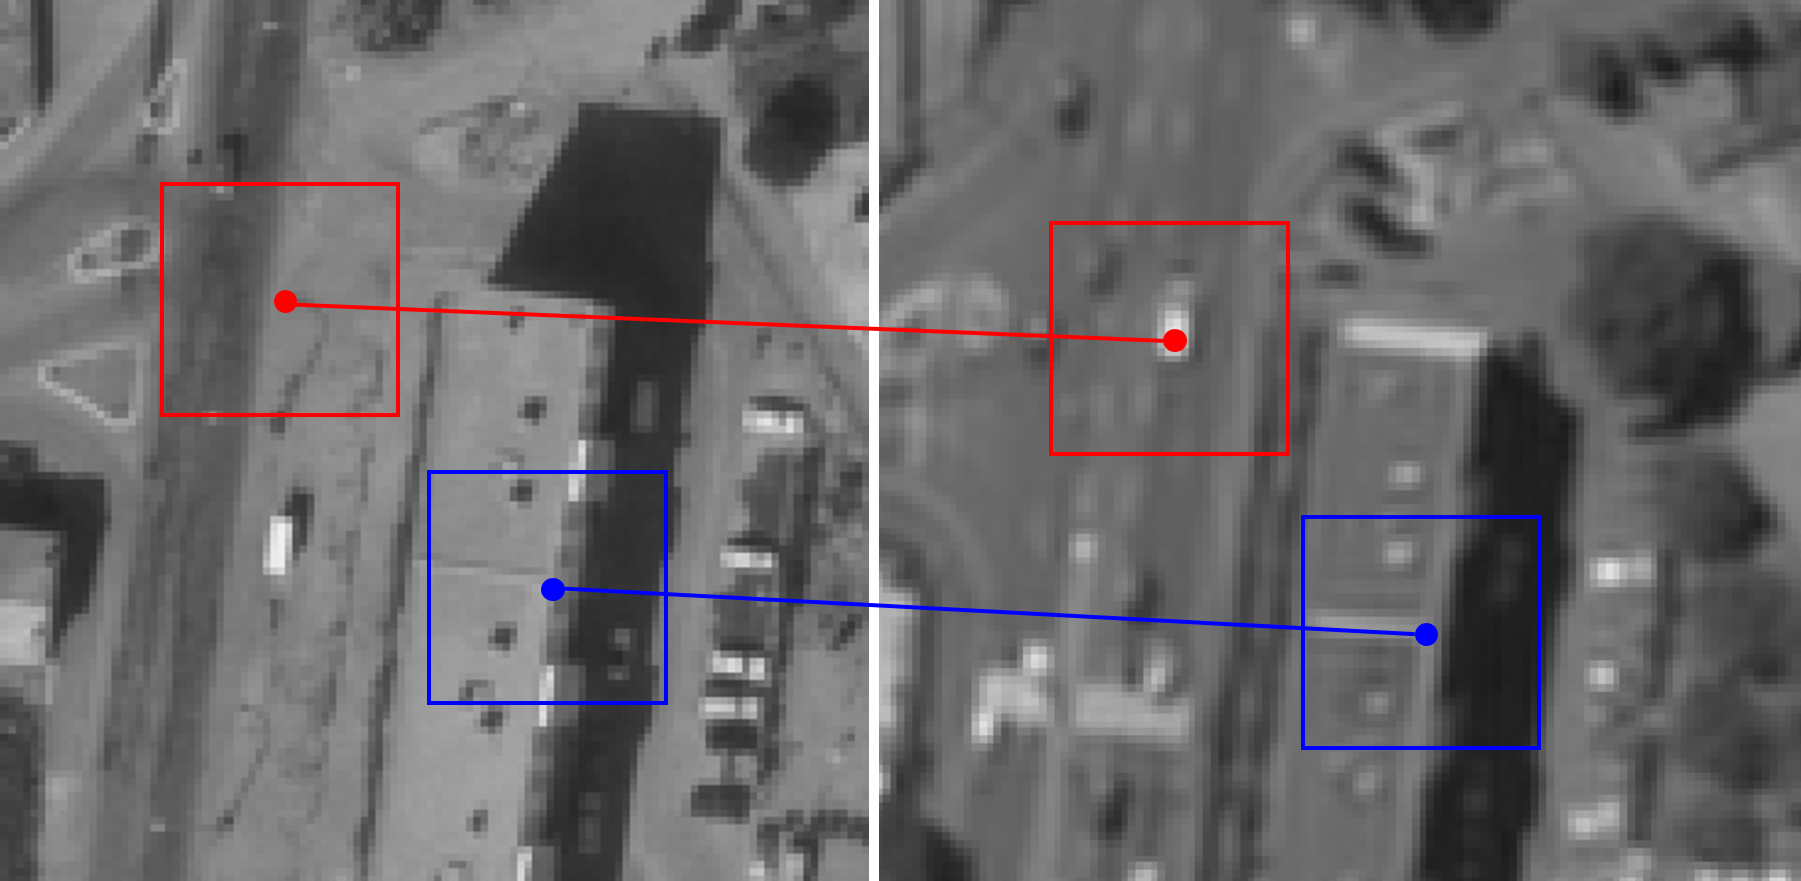
\includegraphics[width=0.8\columnwidth]{images/Chapitre4/tiept.png}
		\caption{Demonstration of the validation with cross-correlation. Considering poor quality of historical images, the window size (blue and red rectangles) was set to 32$\times$32 pixels. False match (red) is eliminated by cross correlation, while true match (blue) is kept.}
		\label{crossc}
	\end{center}
\end{figure*}

\subsection{Refine orientations}
Based on the intra-epoch and inter-epoch matches, a free network \ac{BBA} is performed to refine all the image orientations and camera calibrations. If the results need to be analyzed in a metric scale, a 3D Helmert transformation will be performed to move the refined acquisitions in an arbitrary reference frame to a metric one. If the precise orientations for one of the epochs were known, their parameters will be fixed during the \ac{BBA} and the subsequent 3D Helmert transformation will be skipped.
We adopted the Fraser model ~\cite{fraser1997digital} to calibrate the cameras and allowed image-dependent affine parameters, the remaining parameters were shared among all images.

\section{Experiments}
As described in the previous section, our precise matching stage relies on RGB images and consists of 3 main steps to get the tentative, enhanced and final matches. In Section ~\ref{CompareRGBDSM} we compare the matching results on RGB images and \ac{DSM}s to explain why we choose the former over the latter to perform precise matching.\\
For obtaining tentative matches, there are 2 alternatives (i.e., patch or guided matching), leading to 2 precise matching variants:\\
\begin{enumerate}
	\item \textit{Patch}: recover tentative matches with patch matching, followed by 3D-RANSAC and cross correlation to remove outliers;
	\item \textit{Guided}: same as \textit{Patch}, except replacing patch matching with guided matching.
\end{enumerate}
For each dataset, we choose the rough co-registration results calculated with $SIFT_{DSM}$ and $SuperGlue_{DSM}$ individually (as they are the most robust variants for rough co-registration) to guide the precise matching \textit{Patch} or \textit{Guided}, leading to 4 sets of variants, which are referred to as:\\
\begin{enumerate}
	\item $Patch_{SpGDSM}$
	\item $Guided_{SpGDSM}$
	\item $Patch_{SIFTDSM}$
	\item $Guided_{SIFTDSM}$
\end{enumerate}
We test our precise matching variants on all the multi-epoch datasets which are elaborated in Chapter~\ref{chap:ApplicationsAndDatasets}: Fr{\'e}jus, Pezenas, Kobe and Alberona. The results are demonstrated in Section \ref{Comparisonof6variantsP}.

%We tested our precise matching methods on the 4 sets of datasets: Fr{\'e}jus, Pezenas and Kobe. Details of the datasets are demonstrated in Section~\ref{Datasets}.\\
For Fr{\'e}jus, Kobe and Alberona, we keep all the epochs for experiments, as Fr{\'e}jus displayed drastic scene changes, while Kobe and Alberona witnessed earthquake and landslide individually. 
%For Pezenas, we choose aerial epoch 1971 and satellite epoch 2014 to test our precise matching and ignore other epochs to simplify the processing, since Pezenas is less challenging case.\\
\zll{In Pezenas, less changes are observed. Therefore we maximize the matching difficulty by choosing both aerial and satellite epoch accompanied with the largest time gap (i.e., aerial epoch 1971 and satellite epoch 2014).\\}
The orientations of \ac{GT} epochs (i.e., Pezenas 2014 and Fr{\'e}jus 2014) were treated as fixed during the combined \ac{BBA} since they were accurately known \textit{a-priori}, while all the remaining orientations were considered as free parameters. At first, {interior orientation parameters} were shared among all images. Once stable initial values were known, interior parameters were further refined with image-dependent affine parameters. The affine component of the camera calibration is expected to model the shear of the analog films, at least partially.\\

%In Section ~\ref{CompareRGBDSM} we compared the matching results on RGB images and \ac{DSM}s over the same area. It demonstrates that there are more matches found in \ac{DSM}s which are less precise. As our goal is to recover accurate matches, the RGB images are more suitable than \ac{DSM}s. Besides, it is more efficient as calculating high resolution \ac{DSM}s is computationally demanding.\\

\subsection{Implementation details}
Same as Section ~\ref{Implementationdetails}, all input images are downsampled by a factor of 3 beforehand to improve efficiency except for dataset Alberona. To calculate the \ac{DSM}s, we further downsample the images by a factor of 4 (different from 8 in Section ~\ref{Implementationdetails}), which amounts to a total downsampling factor of 12 with respect to the input images (total factor of 4 for Alberona). For example, the images in Fr{\'e}jus 1970 are downsampled from [8766, 8763] to [730, 730] for calculating \ac{DSM}s. 
Note that the \ac{DSM}s serve 2 purposes in precise matching: (1) narrowing down the search space in \zll{finding tentative matches}, and (2) providing 3D coordinates for 3D-RANSAC filter. A low resolution surface is good enough for these tasks and improves the efficiency.\\
\zll{For patch matching, the buffered tile size $SZ_{one-to-one}$ is set to be 640$\times$480 pixels, the buffer size $SZ_{buffer}$ is 10\%$\times$$SZ_{one-to-one}$ (i.e., widening 64 pixels on both left and right sides, 48 pixels on both upper and lower sides). Therefore, the original tile size $SZ_{one-to-one}^{Orig}$ is left to be 512$\times$384 pixels. The tile pairs entering SuperGlue are not downsampled. For guided matching, the search radius $S$ is set to be 100 pixels. 
For the 3D-RANSAC procedure, we set the number of iteration to 1000, and $T_r$ to 10$\times$$GSD$ where $GSD$ is the mean ground sampling distance in the coordinate frame of reference epoch $E_r$. This distance is computed as the ground distance between two adjacent image pixels. The threshold $T_c$ in cross correlation is set to be 0.6.}
To balance the number of the intra- and inter-epoch matches, we perform intra-epoch matches reduction available as command \textit{Ratafia} in MicMac~\cite{marc2016micmac}. %, with the objective of limiting the number of matches while maintaining a good photogrammetric distribution. 
If the intra-epoch matches after reduction are still obviously more than the inter-epoch ones, we further set the relative observation weight in the \ac{BBA}. The matches reduction algorithm maximizes good spatial distribution, points' multiplicity and low reprojection error, it also helps to speed up the \ac{BBA}.\\
Inter-epoch matches are extracted {for every possible combination of 2 epochs and finally merged}.\\

\subsection{Comparison of precise matching on DSMs and original RGB images}
\label{CompareRGBDSM}
In order to decide which type of image (\ac{DSM} or original RGB image) is more suitable for executing precise matching, we apply our variant \textit{Patch} on both \ac{DSM}s and RGB images of Fr{\'e}jus 1970 and 2014 for comparison.
The final matches are displayed in Figure~\ref{precisematchingdepth} (a) and (b). 
To asses quantitatively the results, we created a \ac{GT} depth map and calculated the accuracy (correct matches / total matches). In Figure~\ref{precisematchingdepth}~(c) we plot the accuracy curves while varying the reprojection error threshold from 0 to 10 pixels. 
Obviously the result using the RGB images is more accurate, even though the \ac{DSM}s recovered more matches.
This is because historical RGB images are inevitably accompanied with noise, and it gets worse in \ac{DSM}s at full resolution (see the \ac{DSM} shaded image in Figure~\ref{precisematchingdepth} (d)) due to inevitably information loss and errors introduction during calculating the \ac{DSM}. Therefore RGB images are more suitable for precise matching.\\
\begin{figure*}[htbp]
	\begin{center}
		\subfigure[Matches on RGB images]{
			\begin{minipage}[t]{0.48\linewidth}
				\centering
				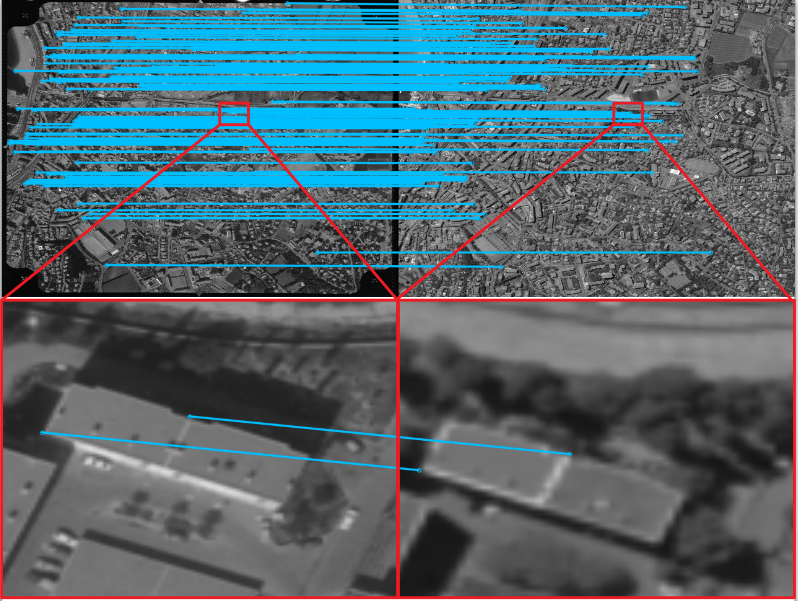
\includegraphics[width=6cm]{images/appendix4/TiePtOriImg.png}
				%\caption{DoD$_{Pezenas\_1971}^{Co-Reg}$}
			\end{minipage}%
		}
		\subfigure[Matches on \ac{DSM}s]{
			\begin{minipage}[t]{0.48\linewidth}
				\centering
				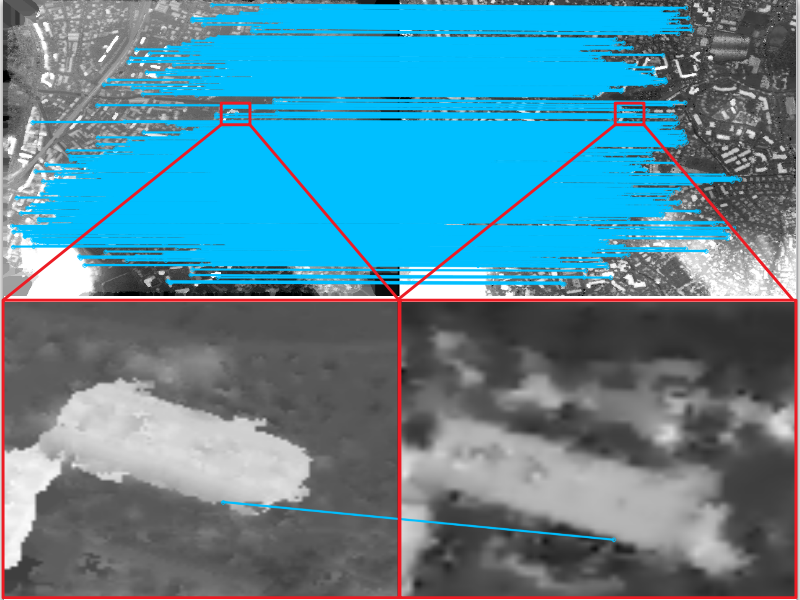
\includegraphics[width=6cm]{images/appendix4/TiePtDepth.png}
				%\caption{DoD$_{Pezenas\_1971}^{Guided}$}
			\end{minipage}  
		}       
		\subfigure[Accuracy of (a) and (b)]{
			\begin{minipage}[t]{0.58\linewidth}
				\centering
				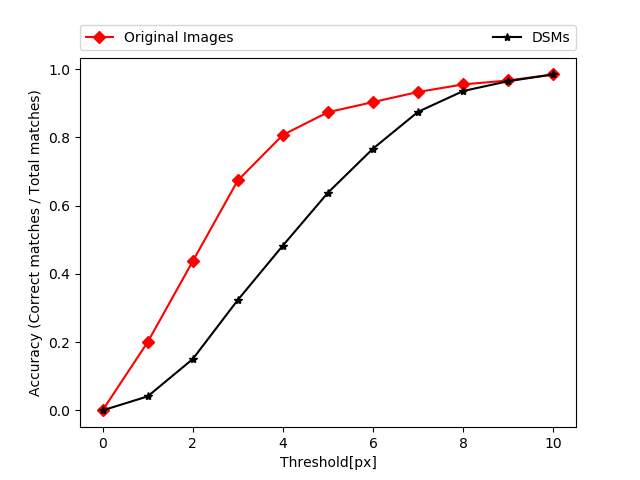
\includegraphics[width=7cm]{images/appendix4/pdfdepth.png}
				%\caption{DoD$_{Pezenas\_1981}^{Co-Reg}$}
			\end{minipage}%
		}
		\subfigure[Shaded image of historical \ac{DSM}]{
			\begin{minipage}[t]{0.38\linewidth}
				\centering
				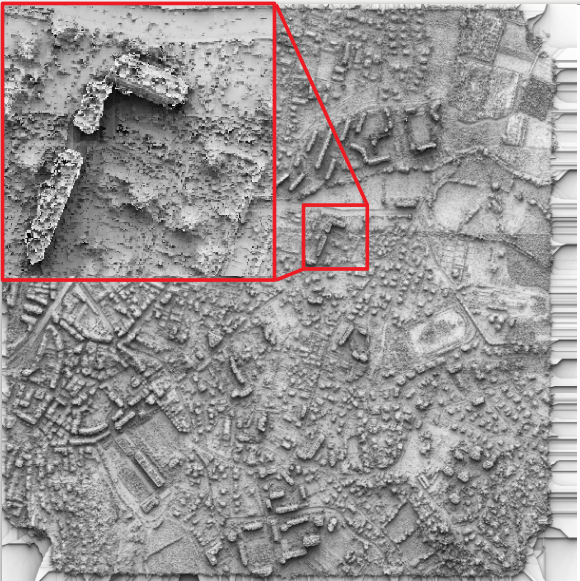
\includegraphics[width=5cm]{images/appendix4/DepthShade.png}
				%\caption{DoD$_{Pezenas\_1981}^{Co-Reg}$}
			\end{minipage}%
		}
		\caption{Comparison of precise matching on original RGB images and \ac{DSM}s.}
		\label{precisematchingdepth}
	\end{center}
\end{figure*} 

%\subsection{Comparison between SIFT and SuperGlue}
%SuperGlue is more invariant over time than SIFT, leading to more numerous matches in the precise matching stage. However, combined with reliable rough co-registration result, SIFT is able to recover less numerous yet more accurate matches than SuperGlue.


%\subsection{Datasets}
%We tested our precise matching variants on all the multi-epoch datasets which are elaborated in Chapter~\ref{chap:ApplicationsAndDatasets}: Fr{\'e}jus, Pezenas, Kobe and Alberona.
%
%%We tested our precise matching methods on the 4 sets of datasets: Fr{\'e}jus, Pezenas and Kobe. Details of the datasets are demonstrated in Section~\ref{Datasets}.\\
%For Fr{\'e}jus, Kobe and Alberona, we keep all the epochs for experiments, as Fr{\'e}jus displayed drastic scene changes, while Kobe and Alberona witnessed earthquake and landslide individually. For Pezenas, we choose aerial epoch 1971 and satellite epoch 2014 to test our precise matching and ignore other epochs to simplify the processing, since Pezenas is less challenging case.\\
%The orientations of \ac{GT} epochs (i.e., Pezenas 2014 and Fr{\'e}jus 2014) were treated as fixed during the combined \ac{BBA} since they were accurately known \textit{a-priori}, while all the remaining orientations were considered as free parameters. At first, {interior orientation parameters} were shared among all images. Once stable initial values were known, interior parameters were further refined with image-dependent affine parameters. The affine component of the camera calibration is expected to model, at least partially, the shear of the analog film.\\
%\subsection{Evaluation}
\subsection{Comparison of 4 variants}
\label{Comparisonof6variantsP}
%Bar chart of recovered match numbers, Match visulization after CC (4 methods, 3 bars each. Kobe and Pezenas: one kit; Frejus: 6 kits)? DoD and statistic info, ground displacment, check pts? 
In order to evaluate the results qualitatively and quantitatively, the following criteria would be applied:\\
%\textcolor{green}{Note: after a detailed comparison with Section \ref{Comparisonof6variants}, the details of Matches visualiation and DoD here are different, so I suggest we leave it like this. What do you think?}
\begin{enumerate}
	\item \textbf{Matches visualization}. The number of tentative, enhanced and final matches are displayed together in bar charts; in the meantime, the final matches are visualized and demonstrated.
	%    \item Ground check points: the co-registered orientations calculated by our methods would be used to triangulate the ground check points and the coordinate differences \textcolor{red}{(explain the diff means the mean diff of x, y and z)} will be displayed. The better the epochs co-register, the smaller the difference is.
	\item \textbf{\ac{DoD}}. For each variant, the refined orientations would be used to calculate \ac{DSM}s in order to generate \ac{DoD}. The visualization of \ac{DoD} as well as the statistical information are displayed. Since the orientations are refined with precise matches, \ac{DoD}s with \textit{dome} effect mitigated or even eliminated are expected.\\
	For Pezenas and Fr{\'e}jus datasets, \ac{DoD}s are calculated between historical epochs and the available \ac{GT} epochs. For Kobe and Alberona datasets, there is no \ac{GT}. Therefore we calculate the \ac{DoD}s between every epochs instead.\\
	%ideally the DoD should only display the scene changes without \textit{dome} effect. If the \textit{dome} effect appears, it indicates the systematic errors caused by poorly estimated camera parameters.   
	\item \textbf{Ground displacement}. For the dataset that witnessed an earthquake (i.e., Kobe), we: (1) calculate the \ac{DSM}s; (2) orthorectify the images; and (3) perform 2D correlation of the respective orthophotos ~\cite{rosu2015measurement} to see whether we can observe the slip of the tectonic plate.
\end{enumerate}

As the results show similar pattern on different datasets, we only display the results of Fr{\'e}jus and Alberona in the current section for the sake of simplicity, and move the results of Kobe as well as Pezenas to Appendix~\ref{chap:appendixB}.\\

%\subsection{Comparison}
%\subsubsection{Matches visualization}
\paragraph{Matches visualization.}
\label{matchVizMainBody}
For each dataset, ze match every possible combination of 2 epochs with 4 variants (i.e., \ding{172} $Patch_{SpGDSM}$, \ding{173} $Guided_{SpGDSM}$, \ding{174} $Patch_{SIFTDSM}$ and \ding{175} $Guided_{SIFTDSM}$). 
%As the matches show similar pattern, for the sake of simplicity, the matches visualizations of datasets Fr{\'e}jus and Alberona are displayed in this chapter, the results of Pezenas and Kobe are demonstrated in Appendix~\ref{sec:PrecisematchViz}.\\

%The matches for dataset Alberona are visualized and displayed in Figure~\ref{MatchVizAlberona}. Matches visualization for datasets Fr{\'e}jus, Pezenas and Kobe are displayed in Section~\ref{chap:appendixB} for the sake of simplicity.\\
%\begin{enumerate}
For Fr{\'e}jus, there exist 4 epochs, leading to 6 sets of epoch combination. The visualizations of resulted matches are displayed in Figure \ref{MatchVizFrejus1954-2014}, \ref{MatchVizFrejus1966-2014}, \ref{MatchVizFrejus1970-2014}, \ref{MatchVizFrejus1954-1970}, \ref{MatchVizFrejus1966-1970} and \ref{MatchVizFrejus1954-1966}.\\
For Alberona, there exist 2 epochs, leading to 1 set of epoch combination, the matches visualization is displayed in Figure~\ref{MatchVizAlberona}.\\
%\end{enumerate}


\begin{figure*}[htbp]
	\begin{center}
		\subfigure[Overlapping zone]{
			\begin{minipage}[t]{0.48\linewidth}
				\centering
				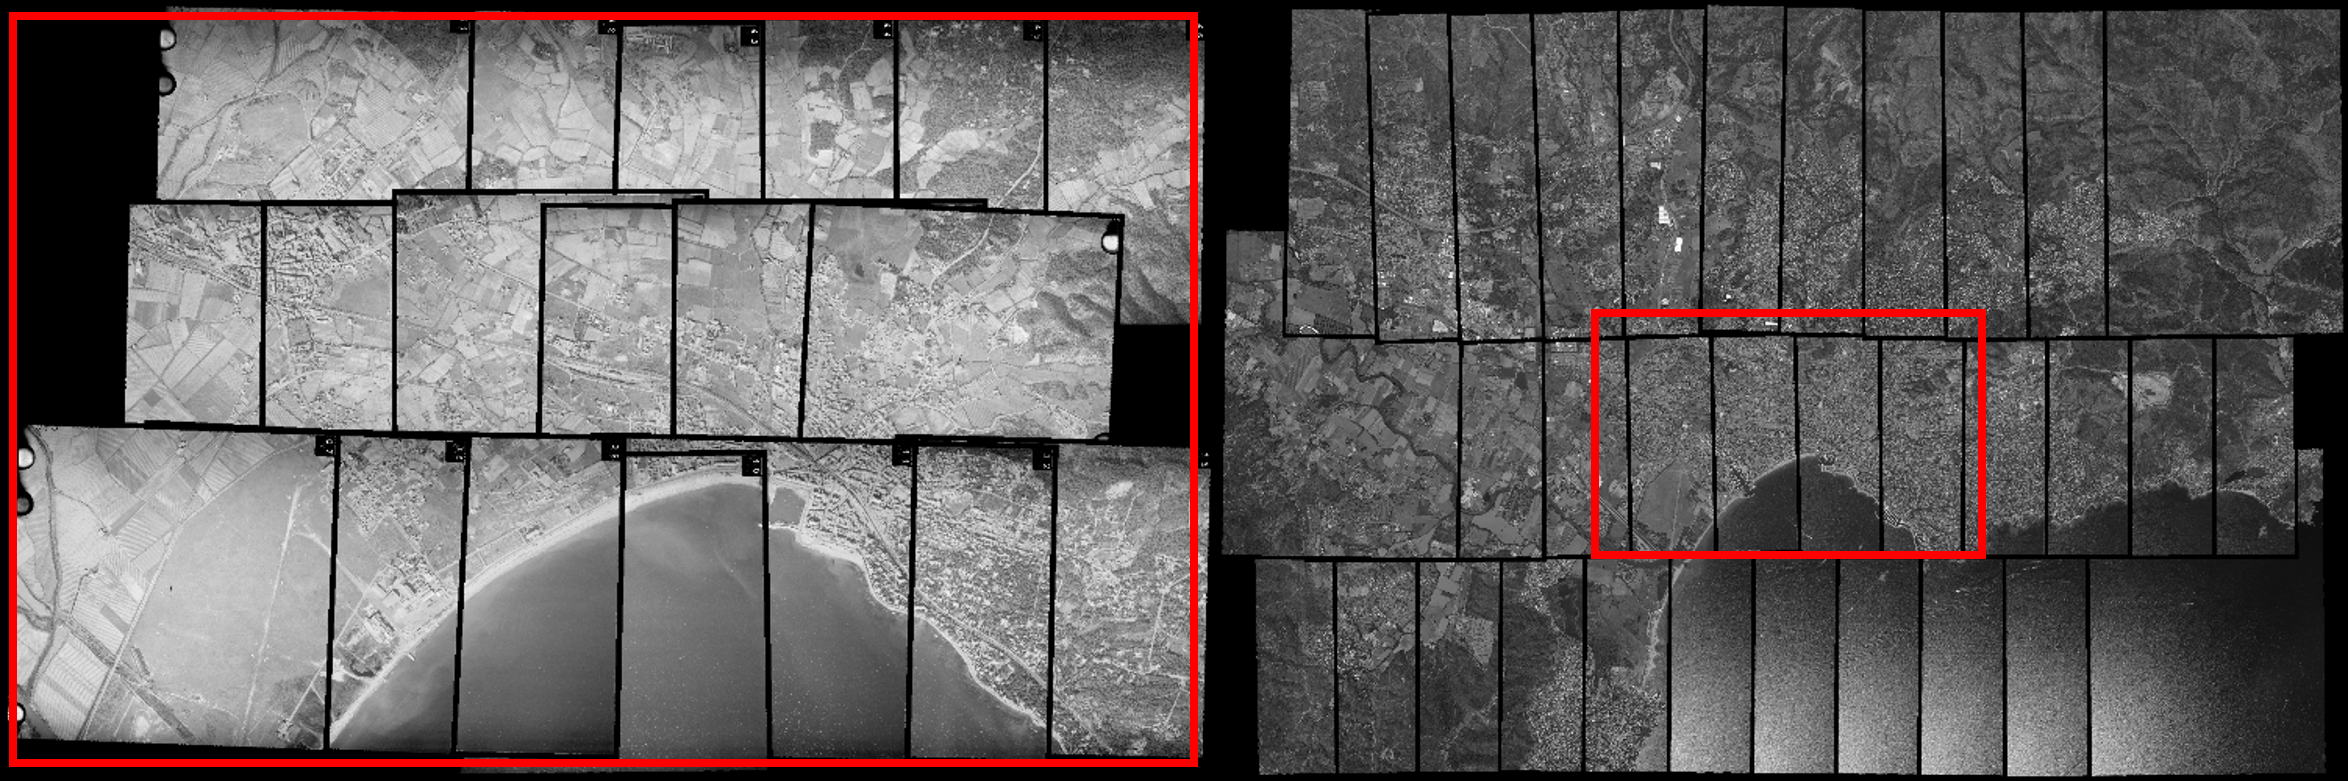
\includegraphics[width=6.8cm]{images/Chapitre3/Pseudo-Ortho-MEC-Malt_Tapas_1954_Ortho-MEC-Malt_2014.png}
			\end{minipage}%
		}
		\subfigure[Number of recovered matches]{
			\begin{minipage}[t]{0.48\linewidth}
				\centering
				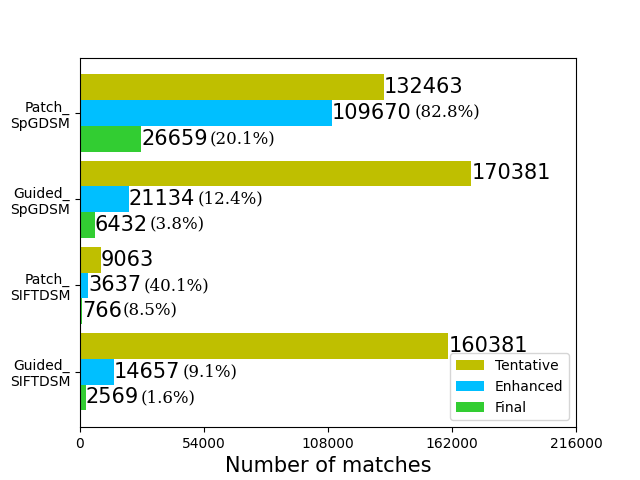
\includegraphics[width=5.8cm]{images/Chapitre4/PlotBarH-Frejus1954-2014.png}
			\end{minipage}%
		}
		\subfigure[$Patch_{SpGDSM}$]{
			\begin{minipage}[t]{0.48\linewidth}
				\centering
				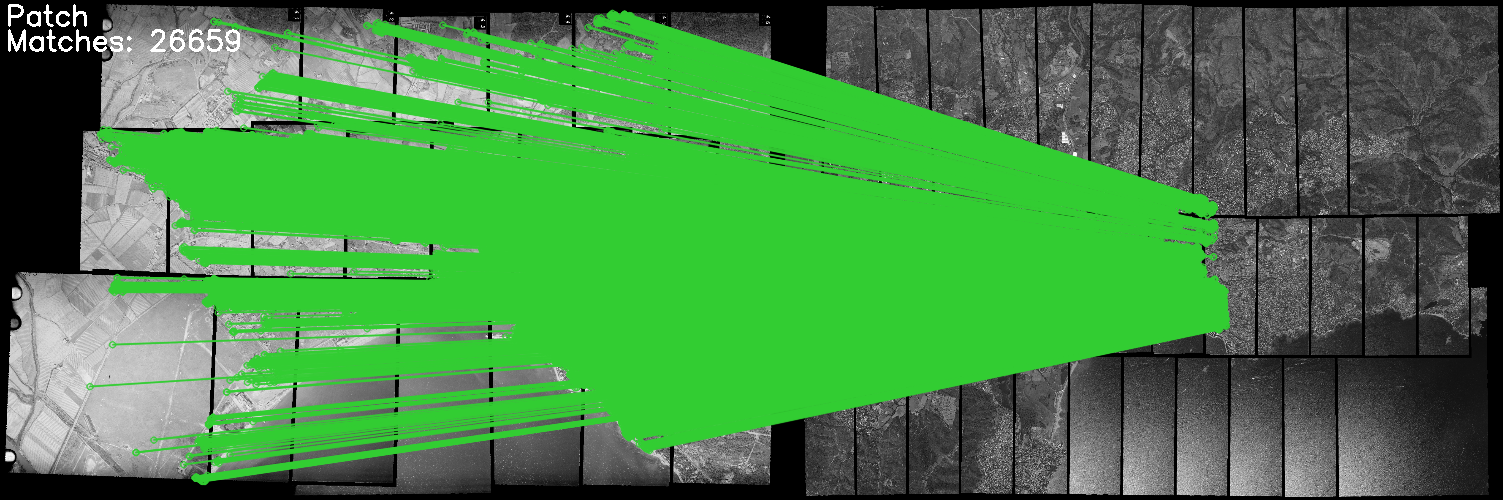
\includegraphics[width=6.8cm]{images/Chapitre4/Precise-SpGDSMHomol-1954-2014-SuperGlue-3DRANSAC-CrossCorrelation-PileImg_Ortho-MEC-Malt_Tapas_1954_Ortho-MEC-Malt_2014.png}
			\end{minipage}%
		}
		\subfigure[$Guided_{SpGDSM}$]{
			\begin{minipage}[t]{0.48\linewidth}
				\centering
				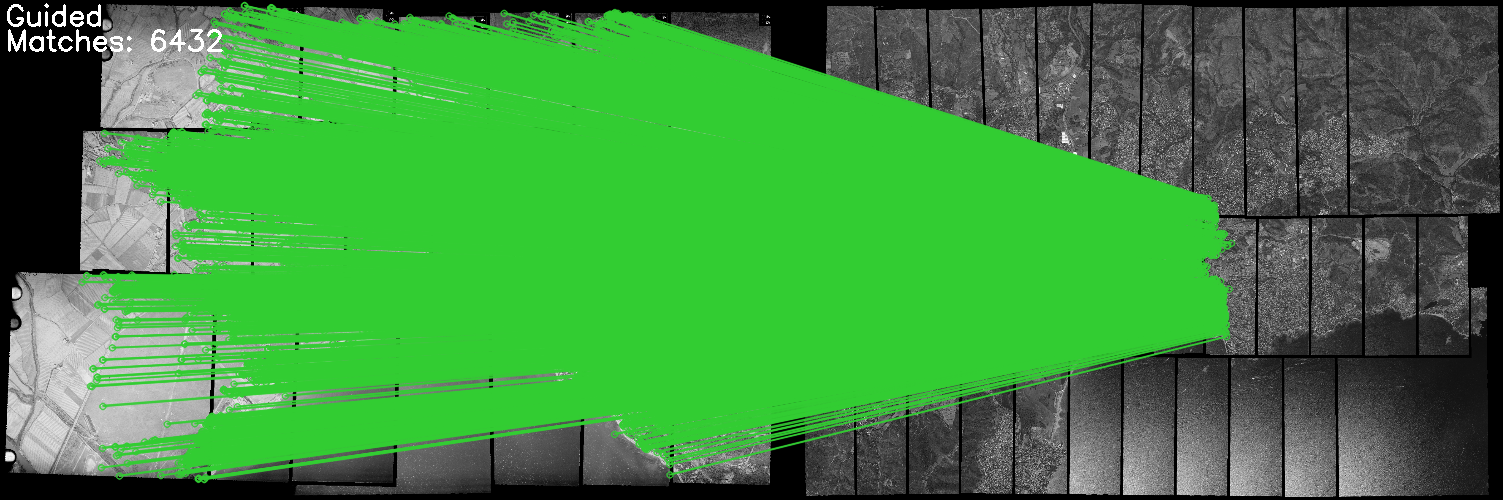
\includegraphics[width=6.8cm]{images/Chapitre4/Precise-SpGDSMHomol-1954-2014-GuidedSIFT-3DRANSAC-CrossCorrelation-PileImg_Ortho-MEC-Malt_Tapas_1954_Ortho-MEC-Malt_2014.png}
			\end{minipage}%
		}
		\subfigure[$Patch_{SIFTDSM}$]{
			\begin{minipage}[t]{0.48\linewidth}
				\centering
				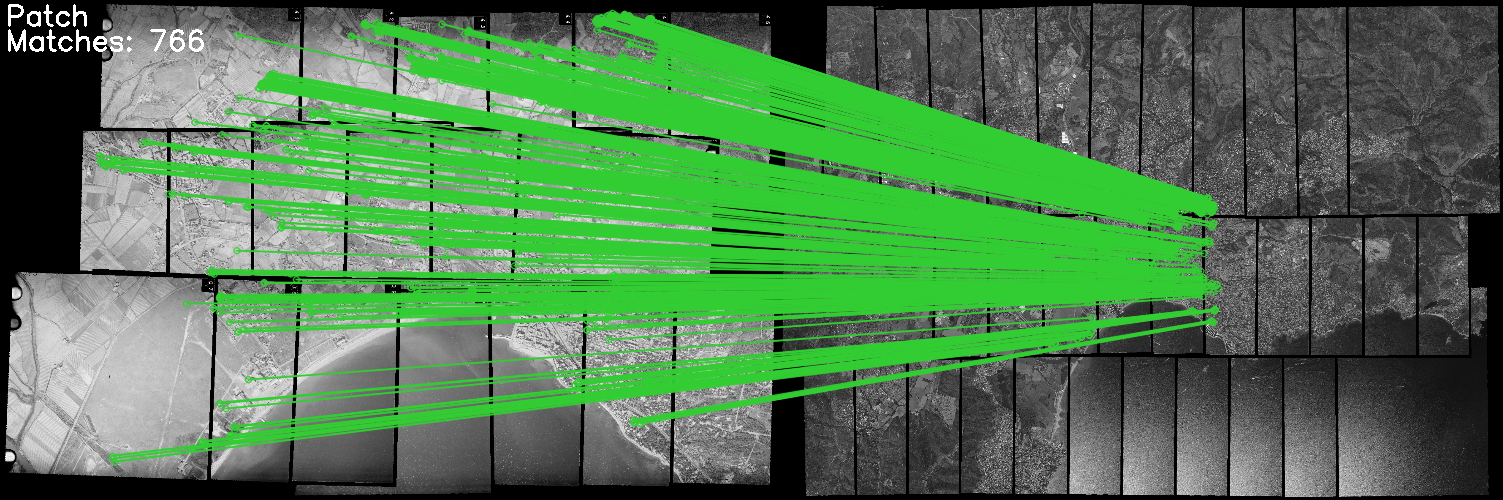
\includegraphics[width=6.8cm]{images/Chapitre4/Precise-SIFTDSMHomol-1954-2014-SuperGlue-3DRANSAC-CrossCorrelation-PileImg_Ortho-MEC-Malt_Tapas_1954_Ortho-MEC-Malt_2014.png}
			\end{minipage}%
		}
		\subfigure[$Guided_{SIFTDSM}$]{
			\begin{minipage}[t]{0.48\linewidth}
				\centering
				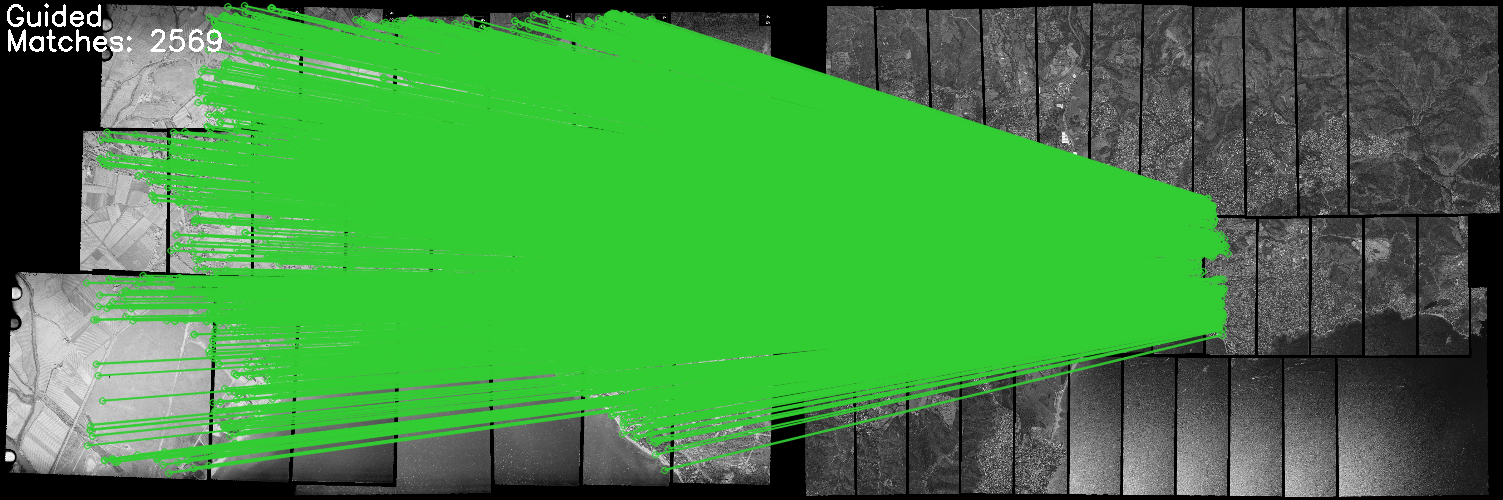
\includegraphics[width=6.8cm]{images/Chapitre4/Precise-SIFTDSMHomol-1954-2014-GuidedSIFT-3DRANSAC-CrossCorrelation-PileImg_Ortho-MEC-Malt_Tapas_1954_Ortho-MEC-Malt_2014.png}
			\end{minipage}%
		}
		\caption{Precise matching visualization of \textbf{Fr{\'e}jus 1954 and 2014}. (a) Image pairs to be matched, with red rectangles indicating the overlapping zone. (b) Numbers of tentative, enhanced and final matches recovered with $Patch_{SpGDSM}$, $Guided_{SpGDSM}$, $Patch_{SIFTDSM}$ and $Guided_{SIFTDSM}$ individually. (c-f) Visualization of final matches recovered with $Patch_{SpGDSM}$, $Guided_{SpGDSM}$, $Patch_{SIFTDSM}$ and $Guided_{SIFTDSM}$ individually.}
		\label{MatchVizFrejus1954-2014}
	\end{center}
\end{figure*} 


\begin{figure*}[htbp]
	\begin{center}
		\subfigure[Overlapping zone]{
			\begin{minipage}[t]{0.48\linewidth}
				\centering
				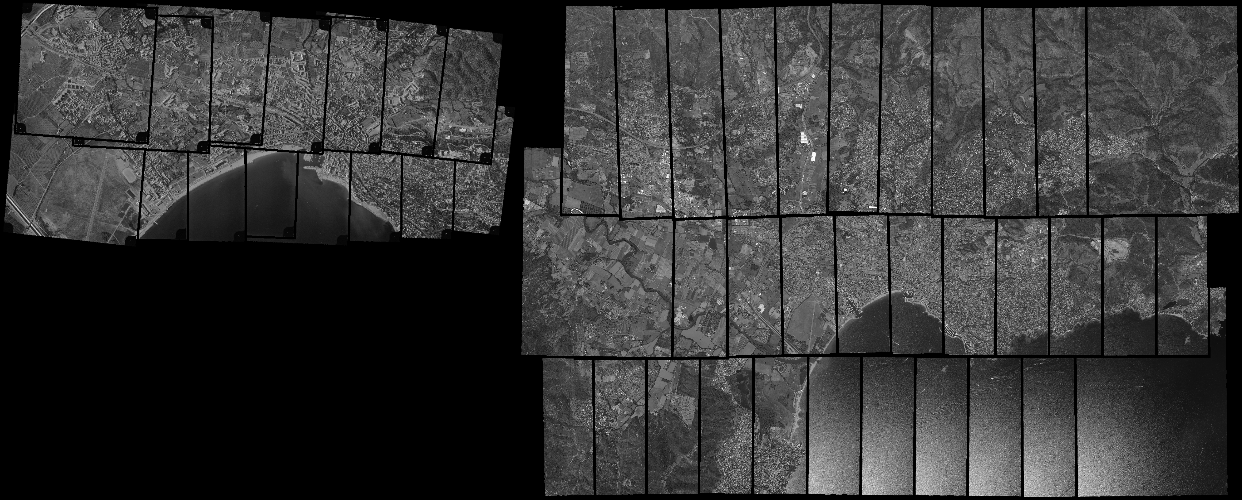
\includegraphics[width=6.8cm]{images/Chapitre3/Pseudo-Ortho-MEC-Malt_Tapas_1966_Ortho-MEC-Malt_2014.png}
			\end{minipage}%
		}
		\subfigure[Number of recovered matches]{
			\begin{minipage}[t]{0.48\linewidth}
				\centering
				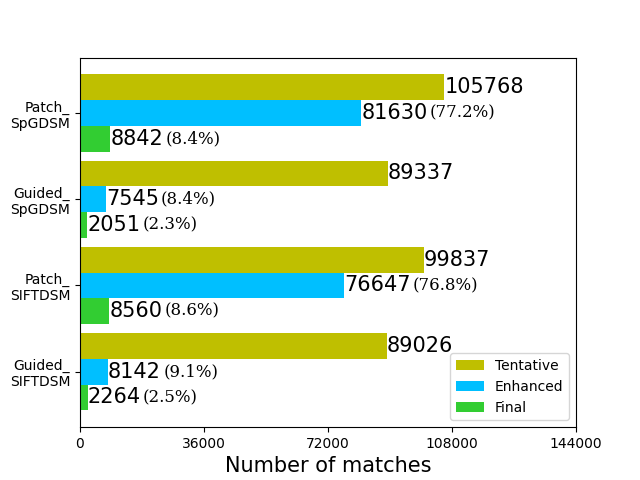
\includegraphics[width=5.8cm]{images/Chapitre4/PlotBarH-Frejus1966-2014.png}
			\end{minipage}%
		}
		\subfigure[$Patch_{SpGDSM}$]{
			\begin{minipage}[t]{0.48\linewidth}
				\centering
				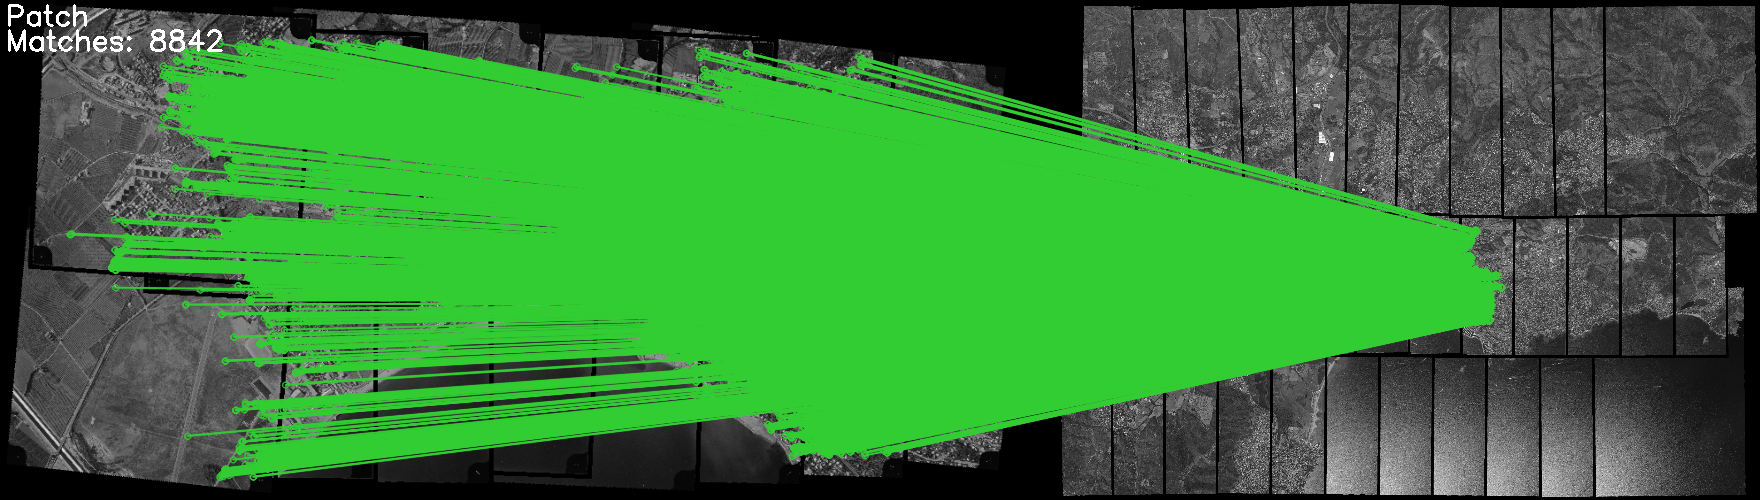
\includegraphics[width=6.8cm]{images/Chapitre4/Precise-SpGDSMHomol-1966-2014-SuperGlue-3DRANSAC-CrossCorrelation-PileImg_Ortho-MEC-Malt_Tapas_1966_Ortho-MEC-Malt_2014.png}
			\end{minipage}%
		}
		\subfigure[$Guided_{SpGDSM}$]{
			\begin{minipage}[t]{0.48\linewidth}
				\centering
				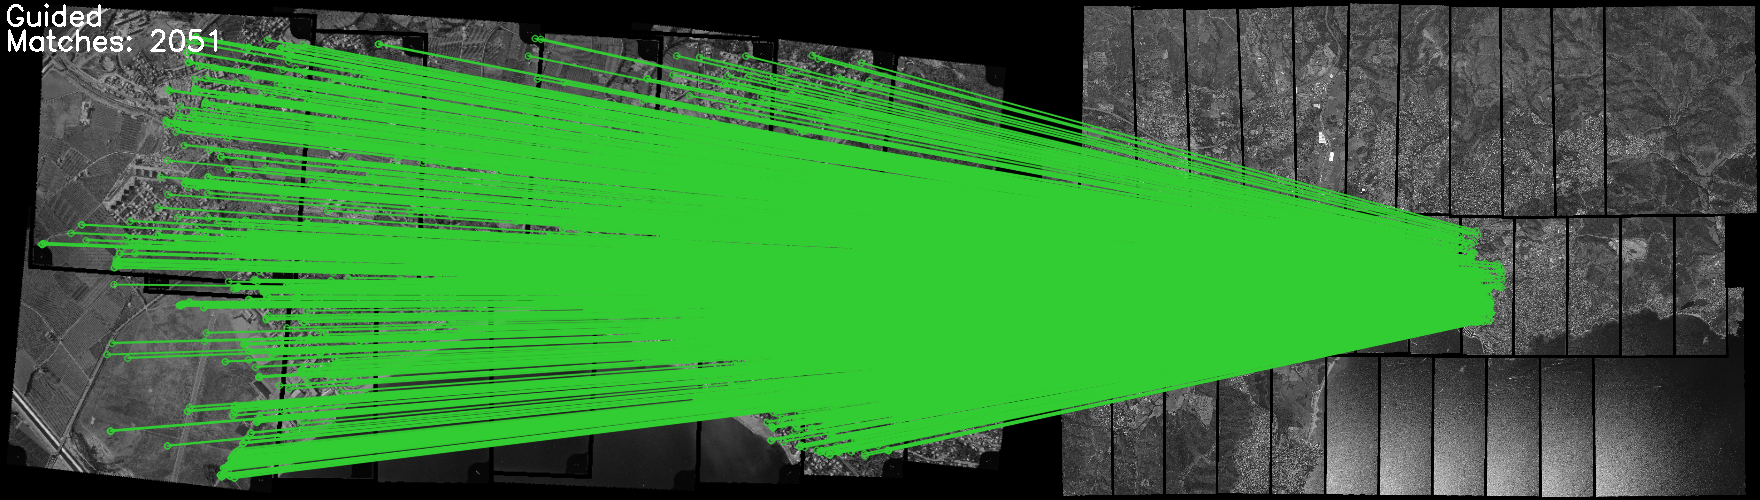
\includegraphics[width=6.8cm]{images/Chapitre4/Precise-SpGDSMHomol-1966-2014-GuidedSIFT-3DRANSAC-CrossCorrelation-PileImg_Ortho-MEC-Malt_Tapas_1966_Ortho-MEC-Malt_2014.png}
			\end{minipage}%
		}
		\subfigure[$Patch_{SIFTDSM}$]{
			\begin{minipage}[t]{0.48\linewidth}
				\centering
				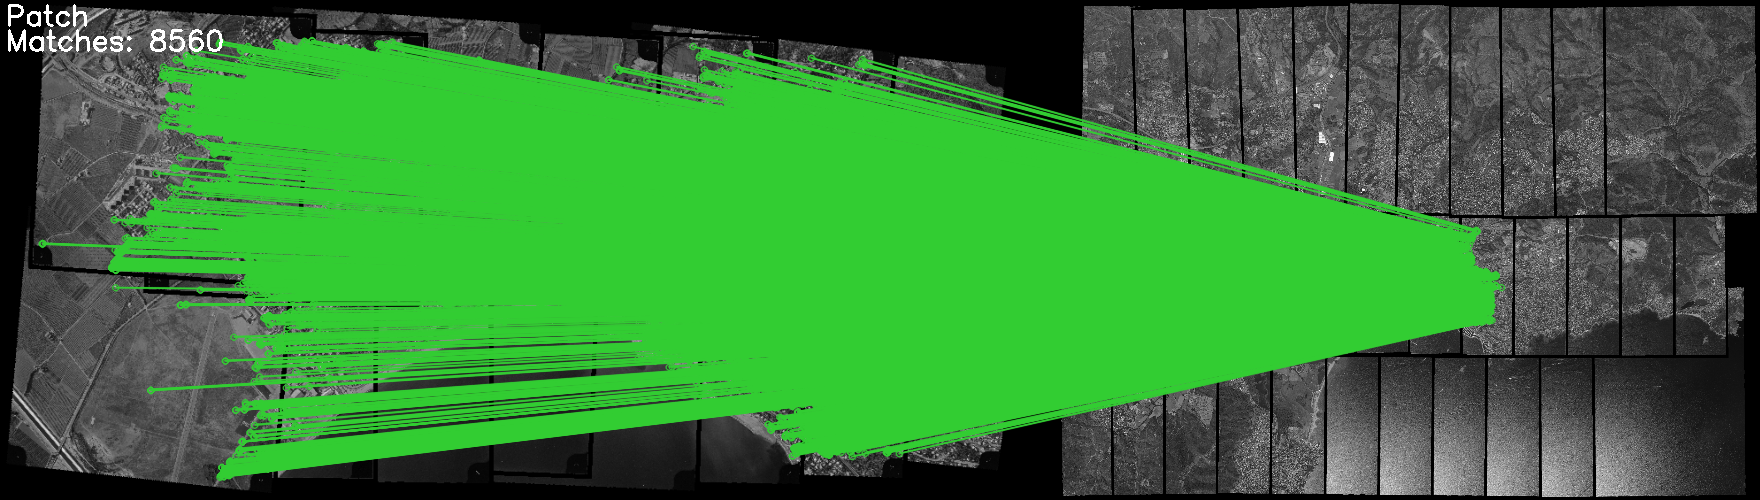
\includegraphics[width=6.8cm]{images/Chapitre4/Precise-SIFTDSMHomol-1966-2014-SuperGlue-3DRANSAC-CrossCorrelation-PileImg_Ortho-MEC-Malt_Tapas_1966_Ortho-MEC-Malt_2014.png}
			\end{minipage}%
		}
		\subfigure[$Guided_{SIFTDSM}$]{
			\begin{minipage}[t]{0.48\linewidth}
				\centering
				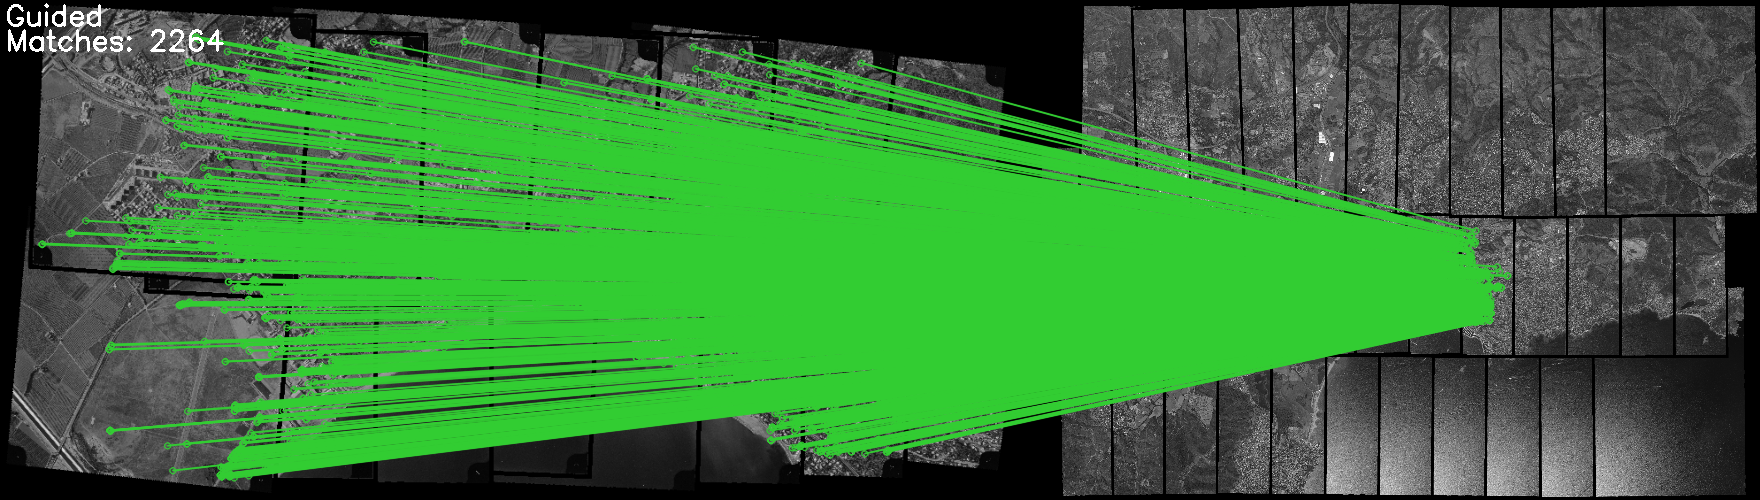
\includegraphics[width=6.8cm]{images/Chapitre4/Precise-SIFTDSMHomol-1966-2014-GuidedSIFT-3DRANSAC-CrossCorrelation-PileImg_Ortho-MEC-Malt_Tapas_1966_Ortho-MEC-Malt_2014.png}
			\end{minipage}%
		}
		\caption{Precise matching visualization of \textbf{Fr{\'e}jus 1966 and 2014}. (a) Image pairs to be matched, with red rectangles indicating the overlapping zone. (b) Numbers of tentative, enhanced and final matches recovered with $Patch_{SpGDSM}$, $Guided_{SpGDSM}$, $Patch_{SIFTDSM}$ and $Guided_{SIFTDSM}$ individually. (c-f) Visualization of final matches recovered with $Patch_{SpGDSM}$, $Guided_{SpGDSM}$, $Patch_{SIFTDSM}$ and $Guided_{SIFTDSM}$ individually.}
		\label{MatchVizFrejus1966-2014}
	\end{center}
\end{figure*} 


\begin{figure*}[htbp]
	\begin{center}
		\subfigure[Overlapping zone]{
			\begin{minipage}[t]{0.48\linewidth}
				\centering
				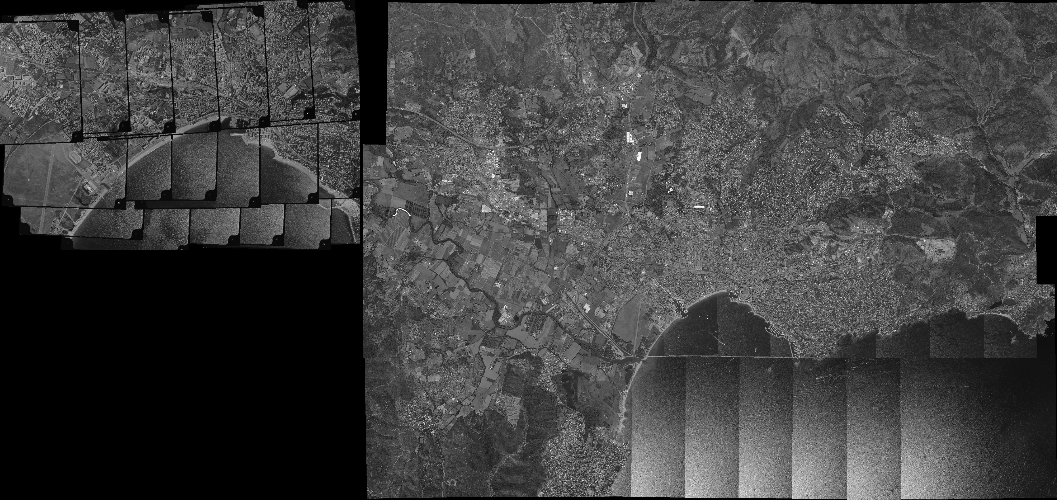
\includegraphics[width=6.8cm]{images/Chapitre3/Pseudo-Ortho-MEC-Malt_Tapas_1970_Ortho-MEC-Malt_2014.png}
			\end{minipage}%
		}
		\subfigure[Number of recovered matches]{
			\begin{minipage}[t]{0.48\linewidth}
				\centering
				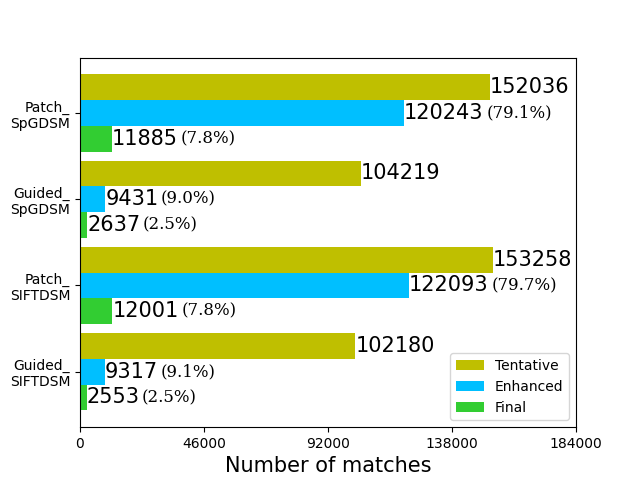
\includegraphics[width=5.8cm]{images/Chapitre4/PlotBarH-Frejus1970-2014.png}
			\end{minipage}%
		}
		\subfigure[$Patch_{SpGDSM}$]{
			\begin{minipage}[t]{0.48\linewidth}
				\centering
				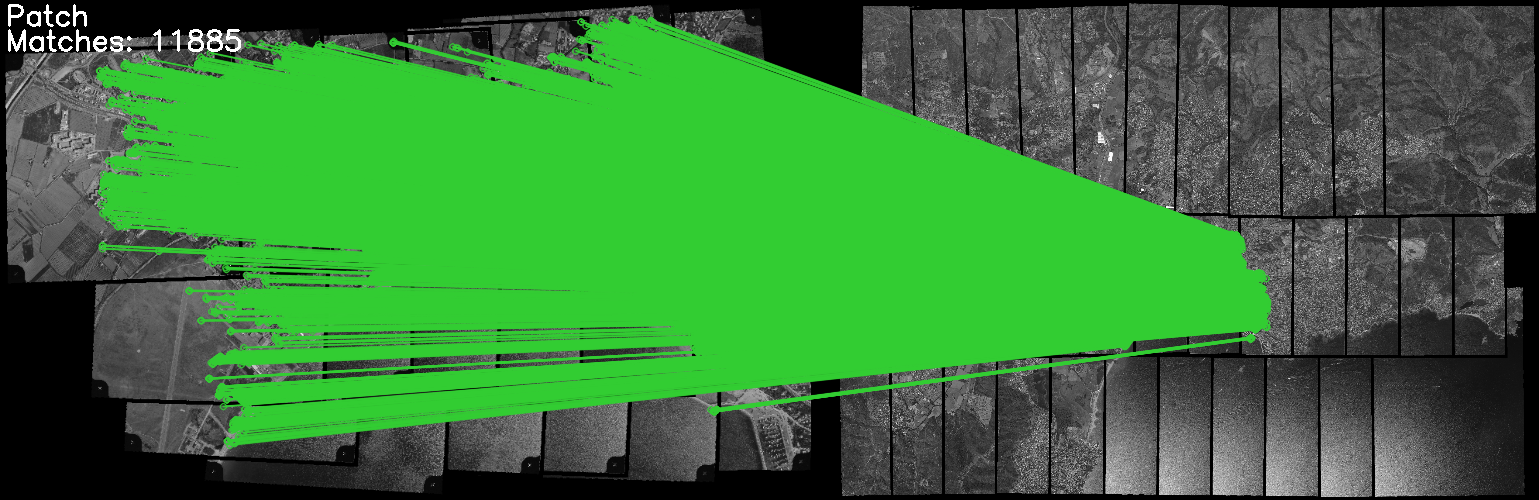
\includegraphics[width=6.8cm]{images/Chapitre4/Precise-SpGDSMHomol-1970-2014-SuperGlue-3DRANSAC-CrossCorrelation-PileImg_Ortho-MEC-Malt_Tapas_1970_Ortho-MEC-Malt_2014.png}
			\end{minipage}%
		}
		\subfigure[$Guided_{SpGDSM}$]{
			\begin{minipage}[t]{0.48\linewidth}
				\centering
				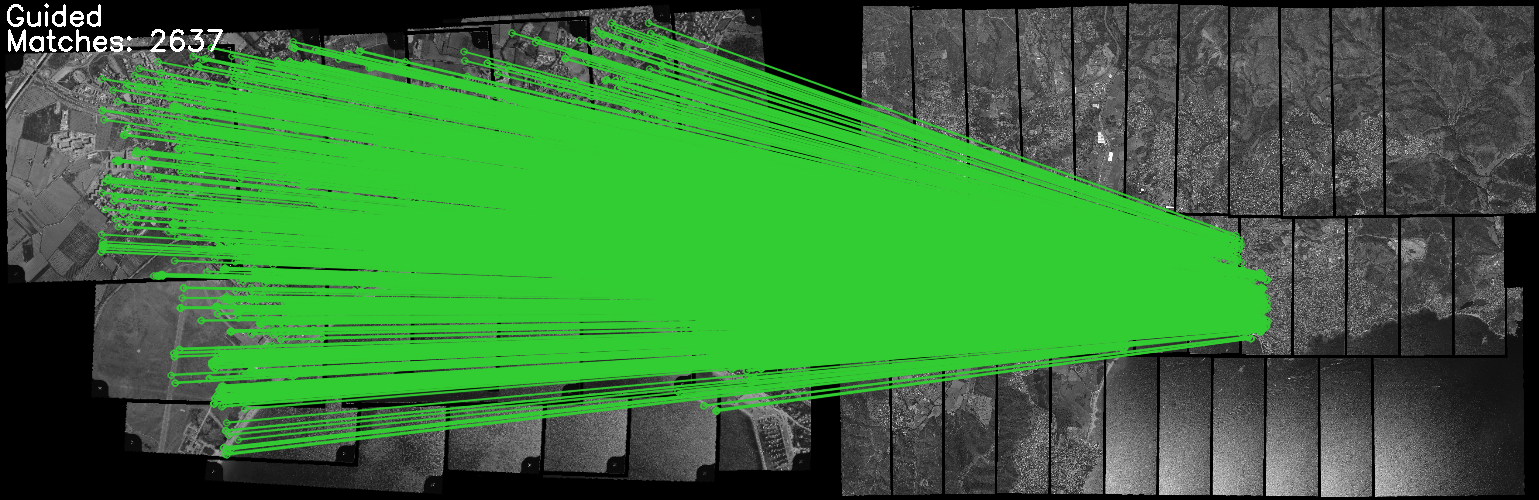
\includegraphics[width=6.8cm]{images/Chapitre4/Precise-SpGDSMHomol-1970-2014-GuidedSIFT-3DRANSAC-CrossCorrelation-PileImg_Ortho-MEC-Malt_Tapas_1970_Ortho-MEC-Malt_2014.png}
			\end{minipage}%
		}
		\subfigure[$Patch_{SIFTDSM}$]{
			\begin{minipage}[t]{0.48\linewidth}
				\centering
				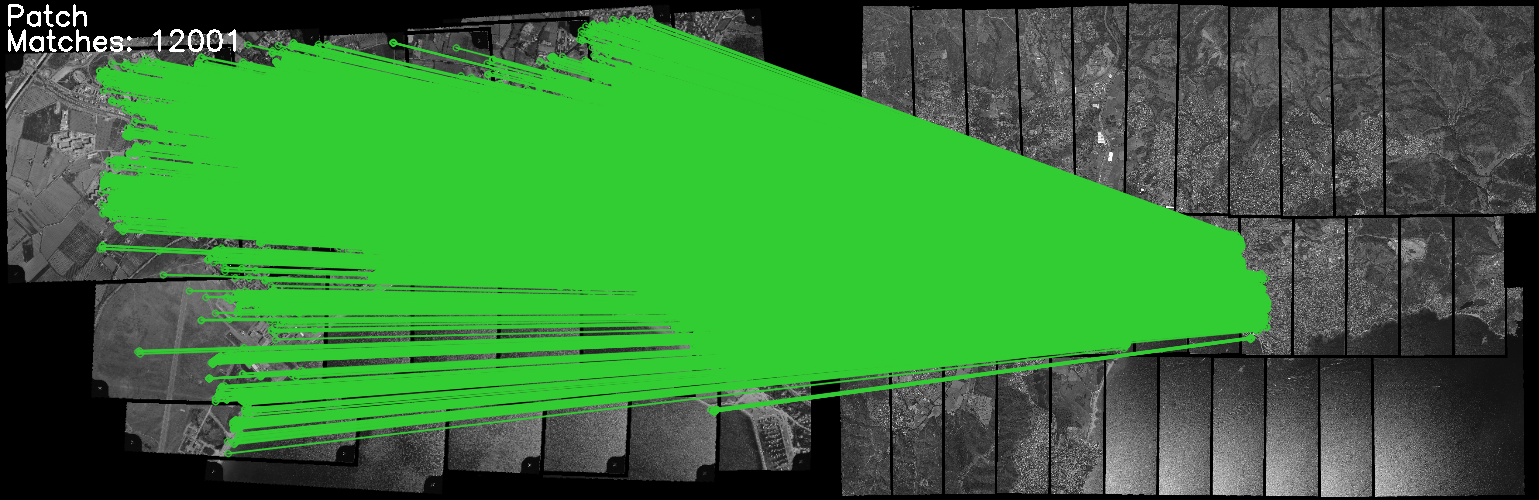
\includegraphics[width=6.8cm]{images/Chapitre4/Precise-SIFTDSMHomol-1970-2014-SuperGlue-3DRANSAC-CrossCorrelation-PileImg_Ortho-MEC-Malt_Tapas_1970_Ortho-MEC-Malt_2014.png}
			\end{minipage}%
		}
		\subfigure[$Guided_{SIFTDSM}$]{
			\begin{minipage}[t]{0.48\linewidth}
				\centering
				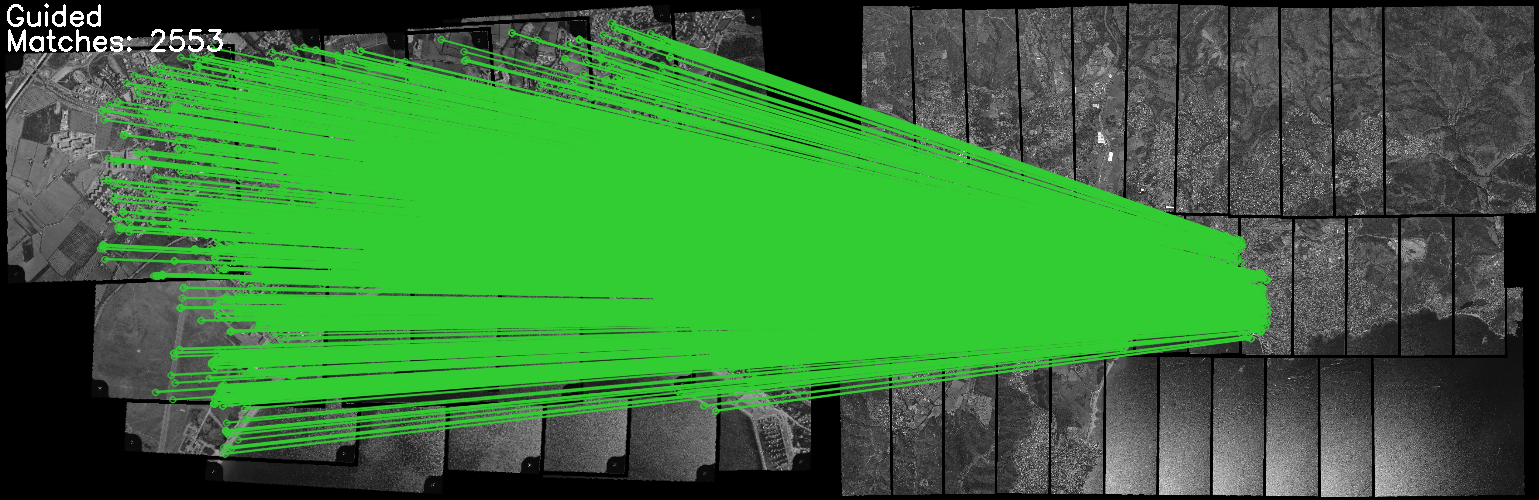
\includegraphics[width=6.8cm]{images/Chapitre4/Precise-SIFTDSMHomol-1970-2014-GuidedSIFT-3DRANSAC-CrossCorrelation-PileImg_Ortho-MEC-Malt_Tapas_1970_Ortho-MEC-Malt_2014.png}
			\end{minipage}%
		}
		\caption{Precise matching visualization of \textbf{Fr{\'e}jus 1970 and 2014}. (a) Image pairs to be matched, with red rectangles indicating the overlapping zone. (b) Numbers of tentative, enhanced and final matches recovered with $Patch_{SpGDSM}$, $Guided_{SpGDSM}$, $Patch_{SIFTDSM}$ and $Guided_{SIFTDSM}$ individually. (c-f) Visualization of final matches recovered with $Patch_{SpGDSM}$, $Guided_{SpGDSM}$, $Patch_{SIFTDSM}$ and $Guided_{SIFTDSM}$ individually.}
		\label{MatchVizFrejus1970-2014}
	\end{center}
\end{figure*} 

%%%%%%%%%%%%%%%%%%Frejus histo

\begin{figure*}[htbp]
	\begin{center}
		\subfigure[Overlapping zone]{
			\begin{minipage}[t]{0.48\linewidth}
				\centering
				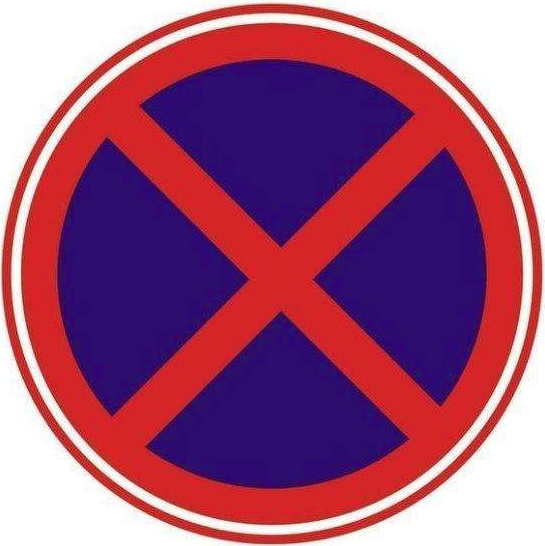
\includegraphics[width=6.8cm]{images/Chapitre4/Pseudo-Ortho-MEC-Malt_Tapas_1954_Ortho-MEC-Malt_Tapas_1970.png}
			\end{minipage}%
		}
		\subfigure[Number of recovered matches]{
			\begin{minipage}[t]{0.48\linewidth}
				\centering
				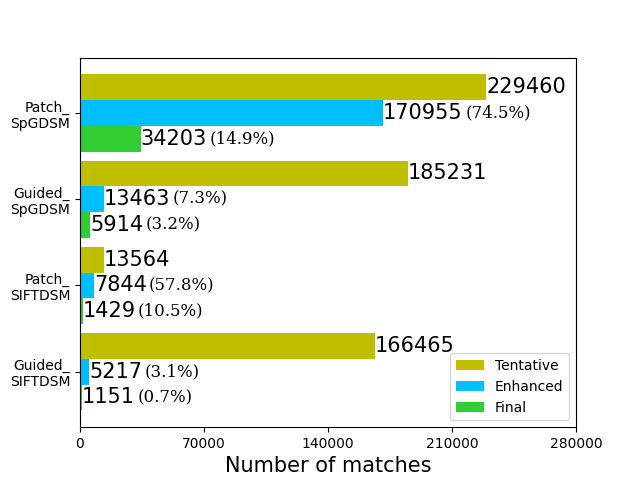
\includegraphics[width=5.8cm]{images/Chapitre4/PlotBarH-Frejus1954-1970.png}
			\end{minipage}%
		}
		\subfigure[$Patch_{SpGDSM}$]{
			\begin{minipage}[t]{0.48\linewidth}
				\centering
				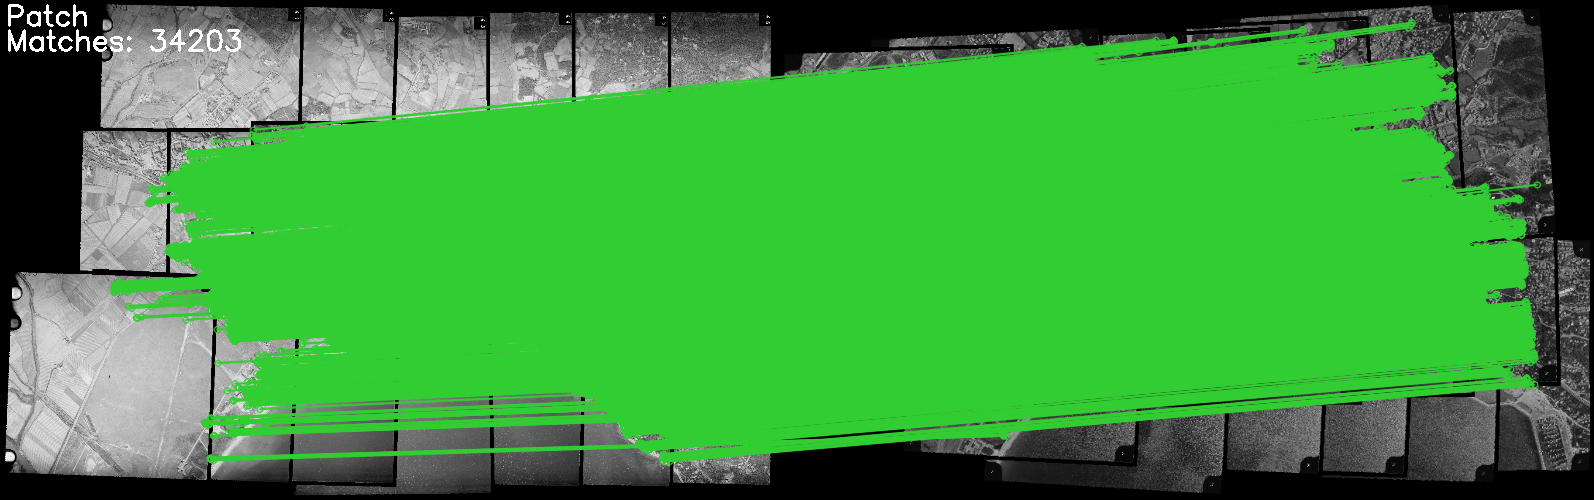
\includegraphics[width=6.8cm]{images/Chapitre4/Precise-SpGDSMHomol-1954-1970-SuperGlue-3DRANSAC-CrossCorrelation-PileImg_Ortho-MEC-Malt_Tapas_1954_Ortho-MEC-Malt_Tapas_1970.png}
			\end{minipage}%
		}
		\subfigure[$Guided_{SpGDSM}$]{
			\begin{minipage}[t]{0.48\linewidth}
				\centering
				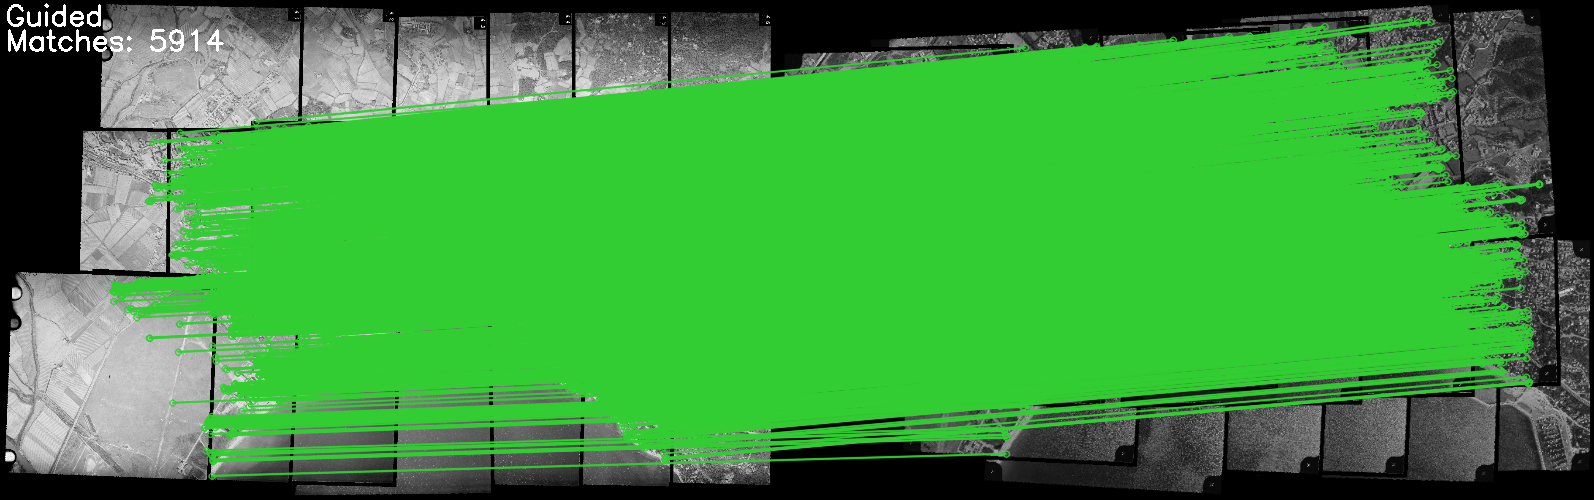
\includegraphics[width=6.8cm]{images/Chapitre4/Precise-SpGDSMHomol-1954-1970-GuidedSIFT-3DRANSAC-CrossCorrelation-PileImg_Ortho-MEC-Malt_Tapas_1954_Ortho-MEC-Malt_Tapas_1970.png}
			\end{minipage}%
		}
		\subfigure[$Patch_{SIFTDSM}$]{
			\begin{minipage}[t]{0.48\linewidth}
				\centering
				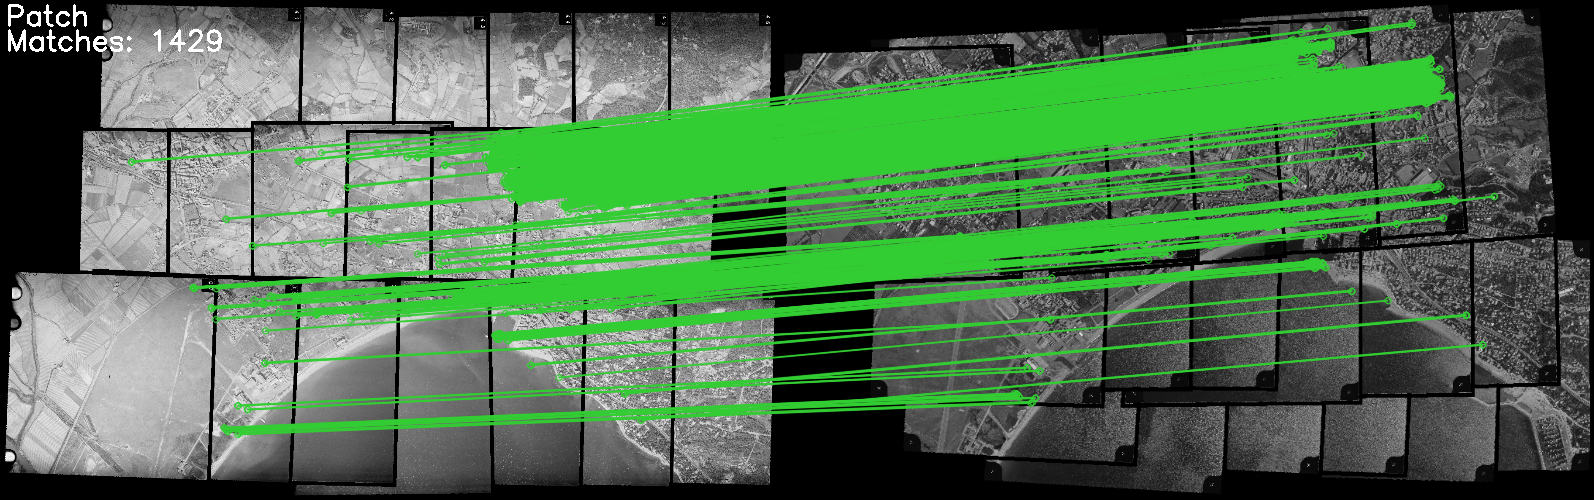
\includegraphics[width=6.8cm]{images/Chapitre4/Precise-SIFTDSMHomol-1954-1970-SuperGlue-3DRANSAC-CrossCorrelation-PileImg_Ortho-MEC-Malt_Tapas_1954_Ortho-MEC-Malt_Tapas_1970.png}
			\end{minipage}%
		}
		\subfigure[$Guided_{SIFTDSM}$]{
			\begin{minipage}[t]{0.48\linewidth}
				\centering
				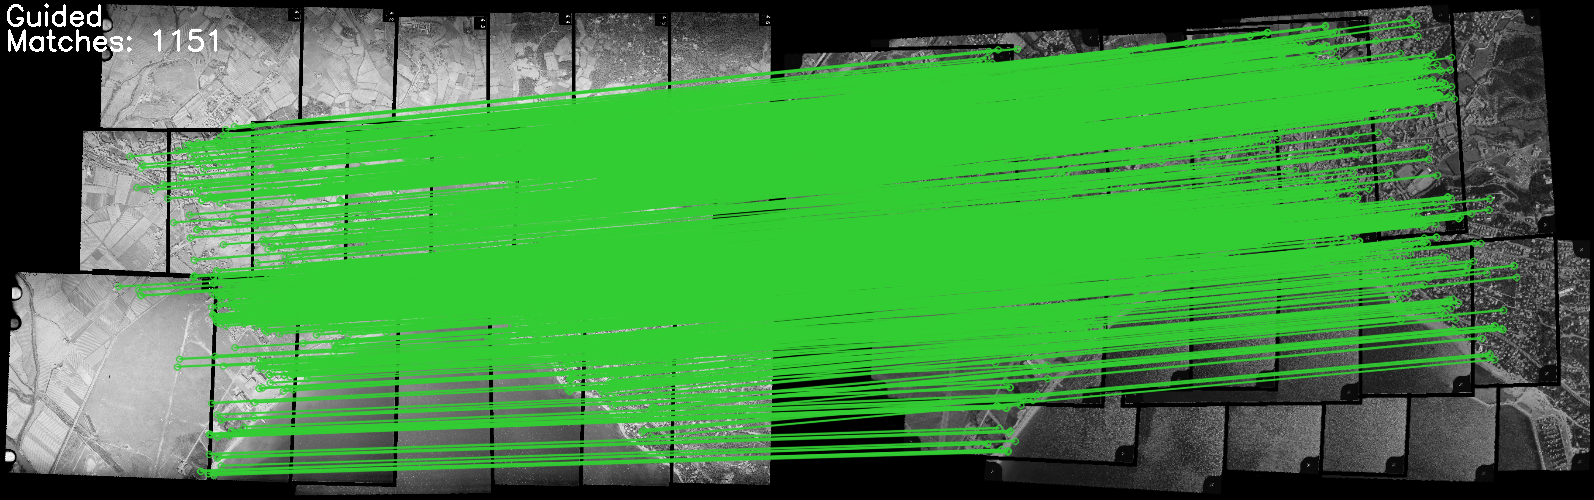
\includegraphics[width=6.8cm]{images/Chapitre4/Precise-SIFTDSMHomol-1954-1970-GuidedSIFT-3DRANSAC-CrossCorrelation-PileImg_Ortho-MEC-Malt_Tapas_1954_Ortho-MEC-Malt_Tapas_1970.png}
			\end{minipage}%
		}
		\caption{Precise matching visualization of \textbf{Fr{\'e}jus 1954 and 1970}. (a) Image pairs to be matched, with red rectangles indicating the overlapping zone. (b) Numbers of tentative, enhanced and final matches recovered with $Patch_{SpGDSM}$, $Guided_{SpGDSM}$, $Patch_{SIFTDSM}$ and $Guided_{SIFTDSM}$ individually. (c-f) Visualization of final matches recovered with $Patch_{SpGDSM}$, $Guided_{SpGDSM}$, $Patch_{SIFTDSM}$ and $Guided_{SIFTDSM}$ individually.}
		\label{MatchVizFrejus1954-1970}
	\end{center}
\end{figure*} 



\begin{figure*}[htbp]
	\begin{center}
		\subfigure[Overlapping zone]{
			\begin{minipage}[t]{0.48\linewidth}
				\centering
				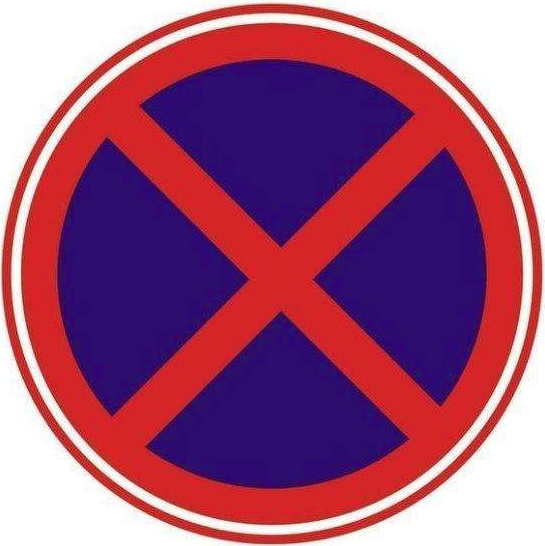
\includegraphics[width=6.8cm]{images/Chapitre4/Pseudo-Ortho-MEC-Malt_Tapas_1966_Ortho-MEC-Malt_Tapas_1970.png}
			\end{minipage}%
		}
		\subfigure[Number of recovered matches]{
			\begin{minipage}[t]{0.48\linewidth}
				\centering
				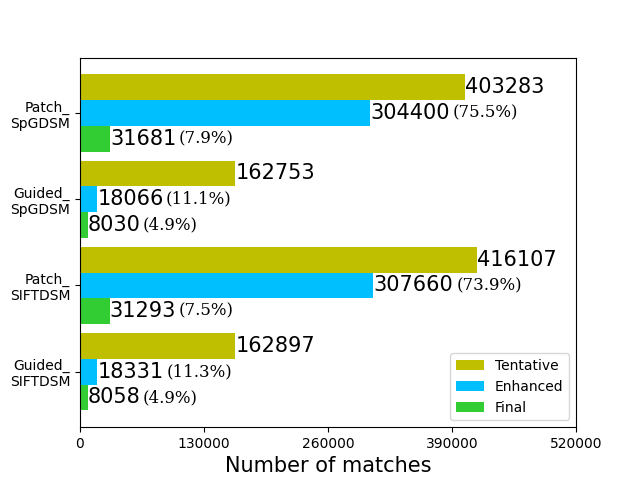
\includegraphics[width=5.8cm]{images/Chapitre4/PlotBarH-Frejus1966-1970.png}
			\end{minipage}%
		}
		\subfigure[$Patch_{SpGDSM}$]{
			\begin{minipage}[t]{0.48\linewidth}
				\centering
				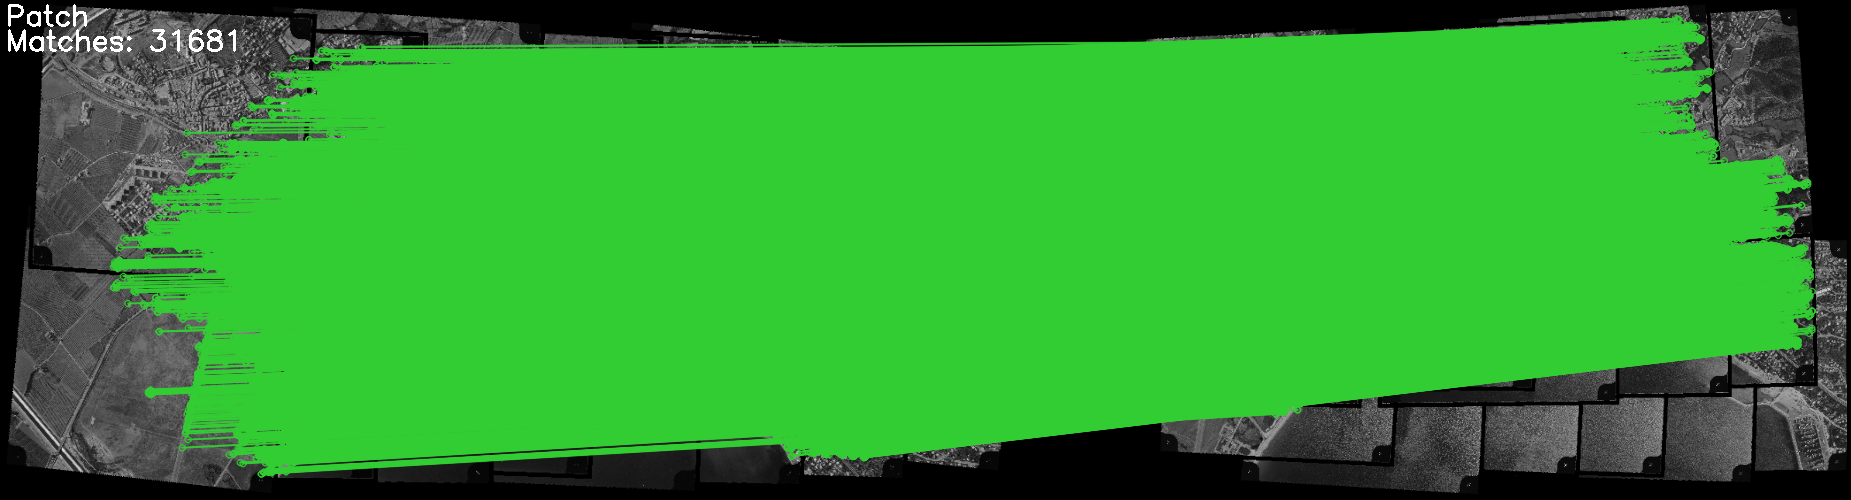
\includegraphics[width=6.8cm]{images/Chapitre4/Precise-SpGDSMHomol-1966-1970-SuperGlue-3DRANSAC-CrossCorrelation-PileImg_Ortho-MEC-Malt_Tapas_1966_Ortho-MEC-Malt_Tapas_1970.png}
			\end{minipage}%
		}
		\subfigure[$Guided_{SpGDSM}$]{
			\begin{minipage}[t]{0.48\linewidth}
				\centering
				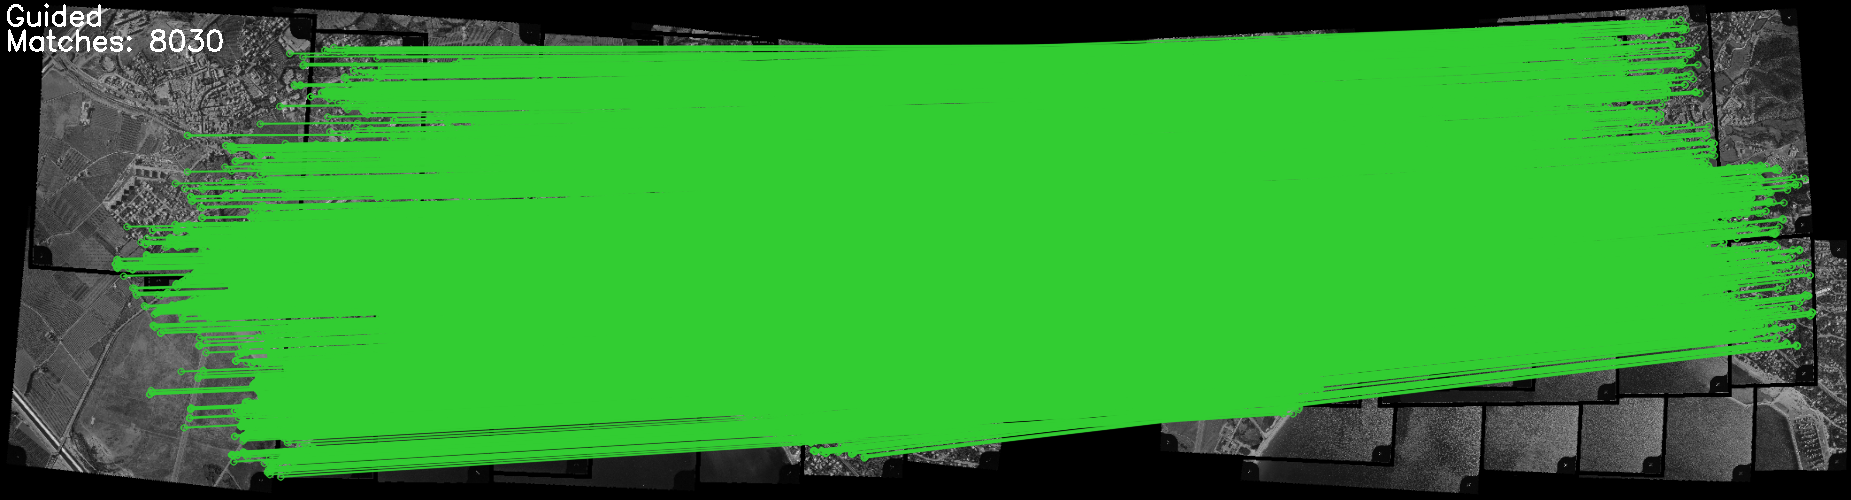
\includegraphics[width=6.8cm]{images/Chapitre4/Precise-SpGDSMHomol-1966-1970-GuidedSIFT-3DRANSAC-CrossCorrelation-PileImg_Ortho-MEC-Malt_Tapas_1966_Ortho-MEC-Malt_Tapas_1970.png}
			\end{minipage}%
		}
		\subfigure[$Patch_{SIFTDSM}$]{
			\begin{minipage}[t]{0.48\linewidth}
				\centering
				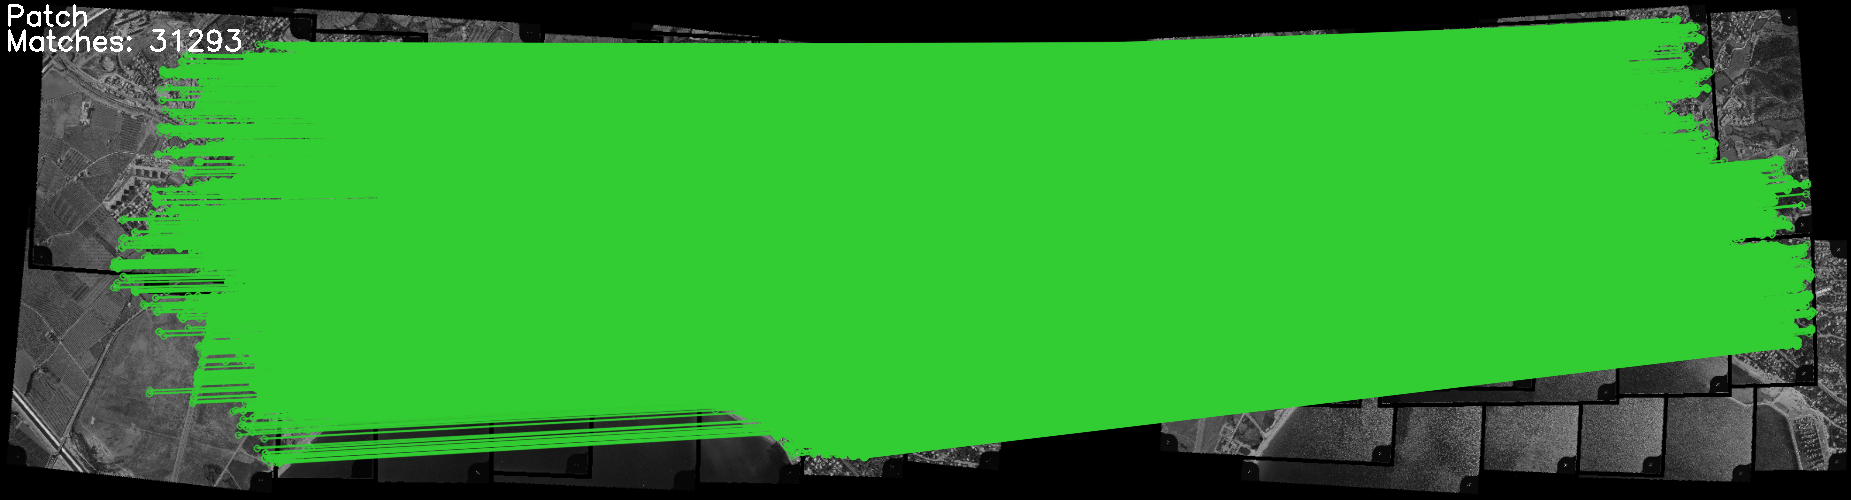
\includegraphics[width=6.8cm]{images/Chapitre4/Precise-SIFTDSMHomol-1966-1970-SuperGlue-3DRANSAC-CrossCorrelation-PileImg_Ortho-MEC-Malt_Tapas_1966_Ortho-MEC-Malt_Tapas_1970.png}
			\end{minipage}%
		}
		\subfigure[$Guided_{SIFTDSM}$]{
			\begin{minipage}[t]{0.48\linewidth}
				\centering
				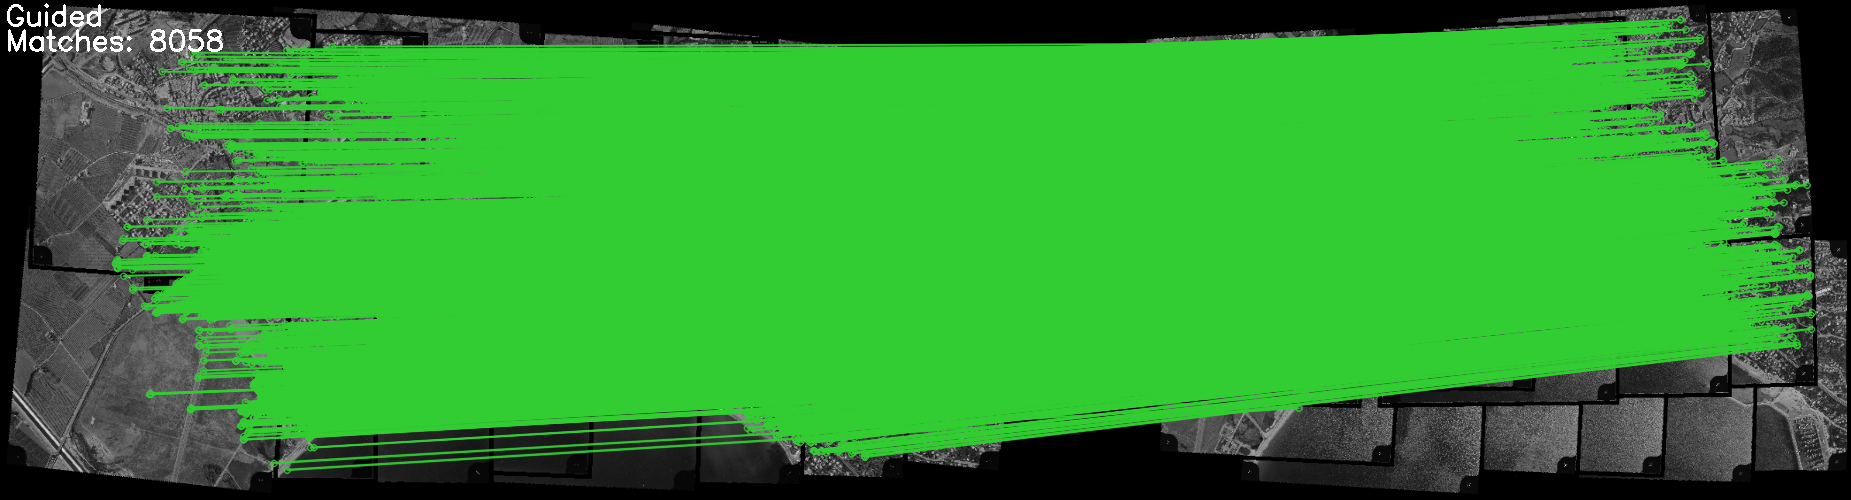
\includegraphics[width=6.8cm]{images/Chapitre4/Precise-SIFTDSMHomol-1966-1970-GuidedSIFT-3DRANSAC-CrossCorrelation-PileImg_Ortho-MEC-Malt_Tapas_1966_Ortho-MEC-Malt_Tapas_1970.png}
			\end{minipage}%
		}
		\caption{Precise matching visualization of \textbf{Fr{\'e}jus 1966 and 1970}. (a) Image pairs to be matched, with red rectangles indicating the overlapping zone. (b) Numbers of tentative, enhanced and final matches recovered with $Patch_{SpGDSM}$, $Guided_{SpGDSM}$, $Patch_{SIFTDSM}$ and $Guided_{SIFTDSM}$ individually. (c-f) Visualization of final matches recovered with $Patch_{SpGDSM}$, $Guided_{SpGDSM}$, $Patch_{SIFTDSM}$ and $Guided_{SIFTDSM}$ individually.}
		\label{MatchVizFrejus1966-1970}
	\end{center}
\end{figure*} 


\begin{figure*}[htbp]
	\begin{center}
		\subfigure[Overlapping zone]{
			\begin{minipage}[t]{0.48\linewidth}
				\centering
				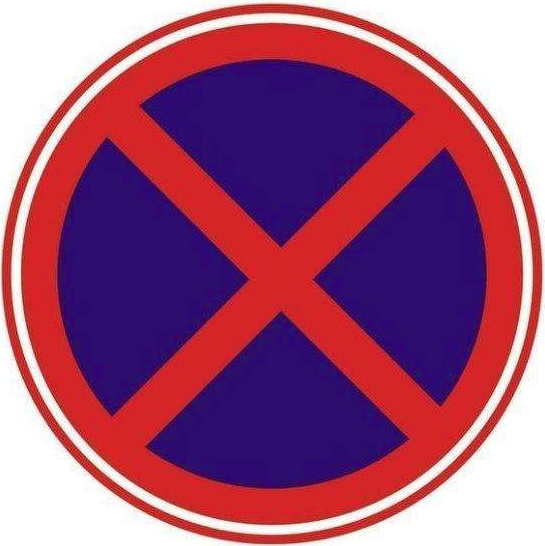
\includegraphics[width=7.8cm]{images/Chapitre4/Pseudo-Ortho-MEC-Malt_Tapas_1954_Ortho-MEC-Malt_Tapas_1966.png}
			\end{minipage}%
		}
		\subfigure[Number of recovered matches]{
			\begin{minipage}[t]{0.48\linewidth}
				\centering
				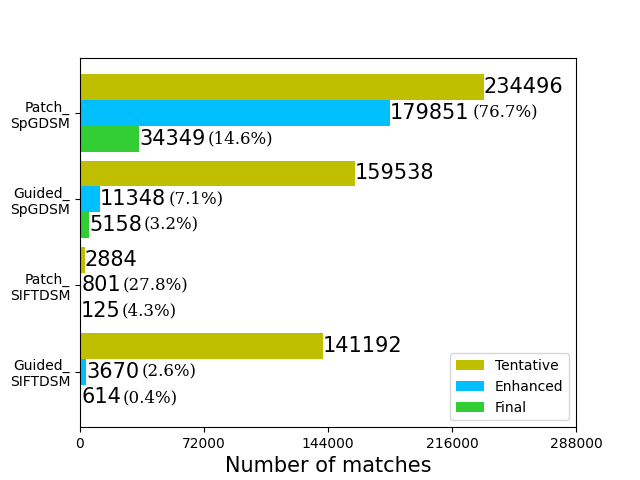
\includegraphics[width=5.8cm]{images/Chapitre4/PlotBarH-Frejus1954-1966.png}
			\end{minipage}%
		}
		\subfigure[$Patch_{SpGDSM}$]{
			\begin{minipage}[t]{0.48\linewidth}
				\centering
				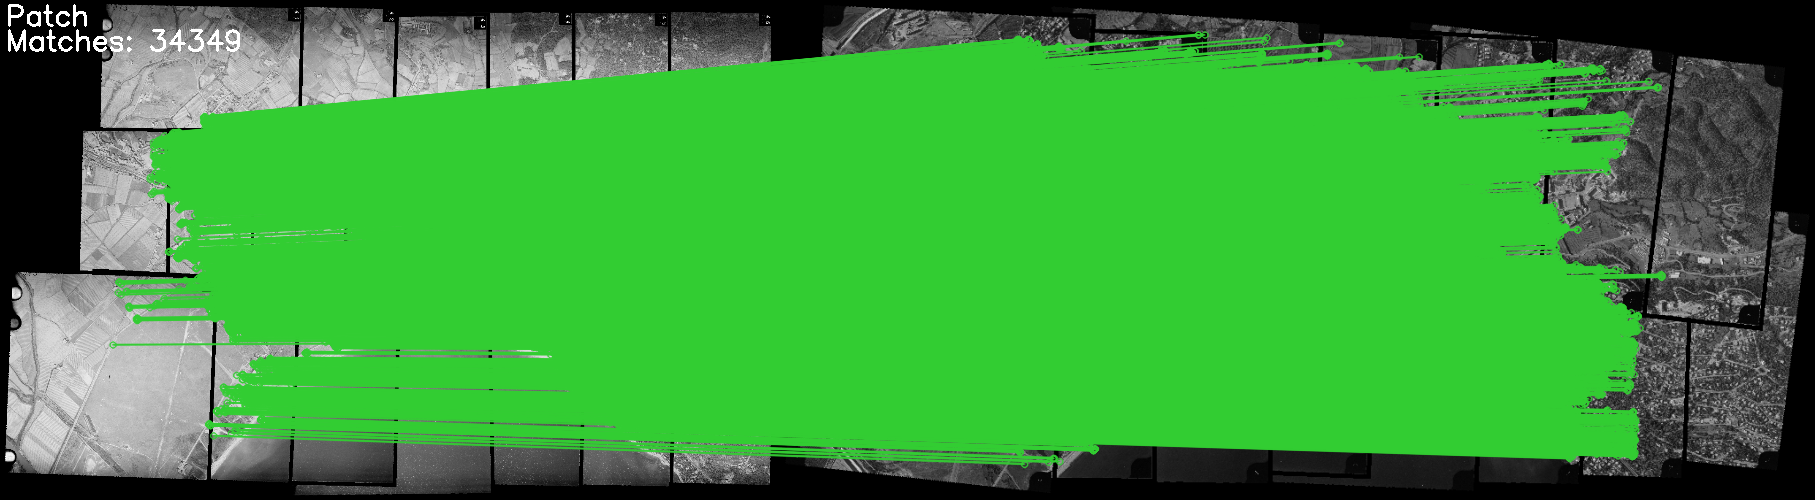
\includegraphics[width=6.8cm]{images/Chapitre4/Precise-SpGDSMHomol-1954-1966-SuperGlue-3DRANSAC-CrossCorrelation-PileImg_Ortho-MEC-Malt_Tapas_1954_Ortho-MEC-Malt_Tapas_1966.png}
			\end{minipage}%
		}
		\subfigure[$Guided_{SpGDSM}$]{
			\begin{minipage}[t]{0.48\linewidth}
				\centering
				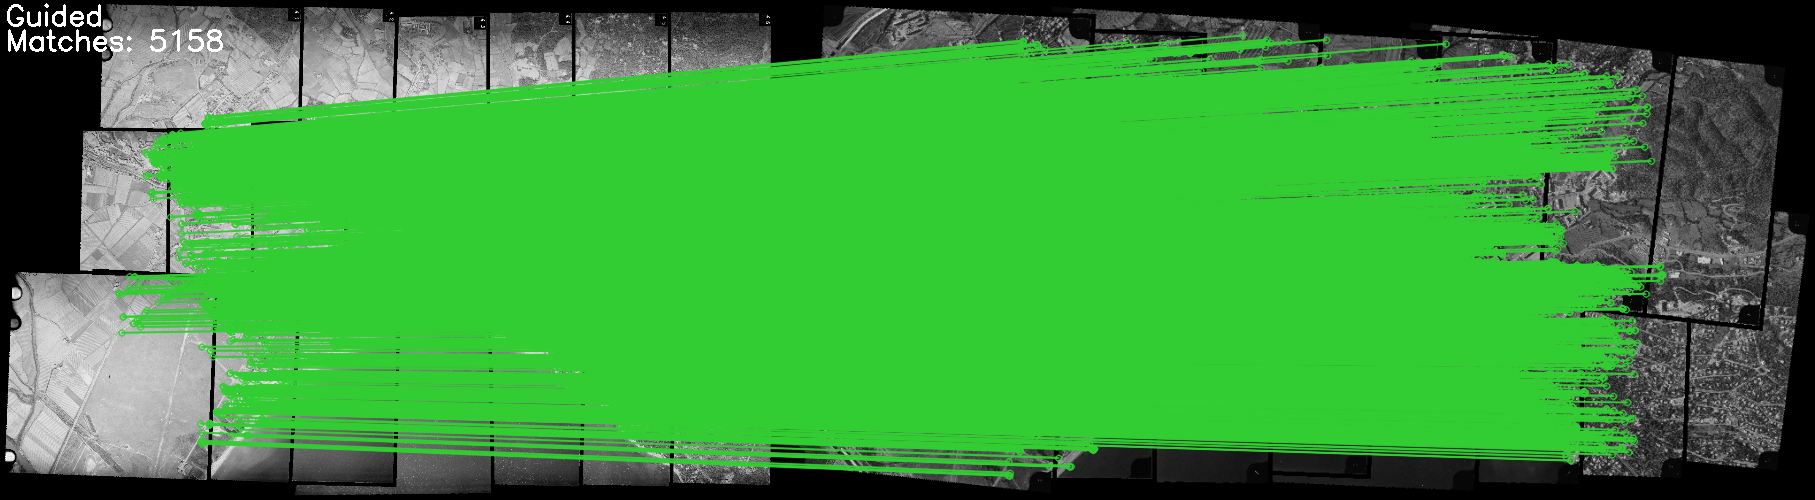
\includegraphics[width=6.8cm]{images/Chapitre4/Precise-SpGDSMHomol-1954-1966-GuidedSIFT-3DRANSAC-CrossCorrelation-PileImg_Ortho-MEC-Malt_Tapas_1954_Ortho-MEC-Malt_Tapas_1966.png}
			\end{minipage}%
		}
		\subfigure[$Patch_{SIFTDSM}$]{
			\begin{minipage}[t]{0.48\linewidth}
				\centering
				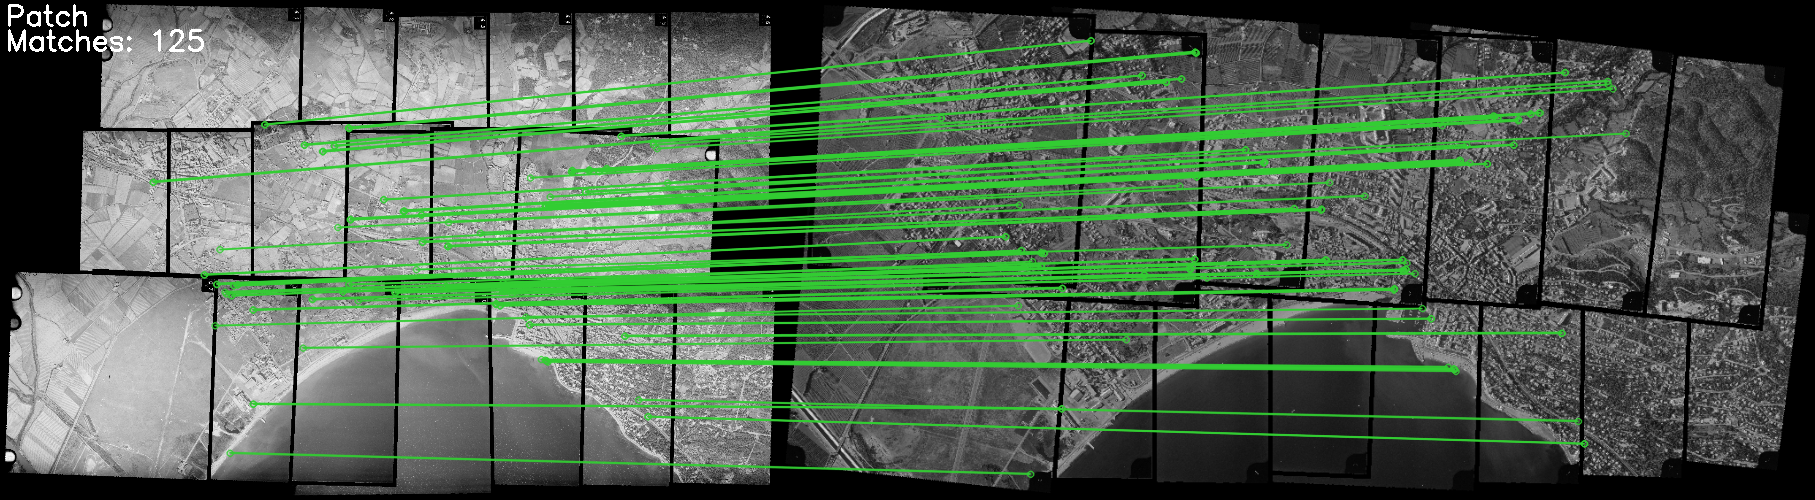
\includegraphics[width=6.8cm]{images/Chapitre4/Precise-SIFTDSMHomol-1954-1966-SuperGlue-3DRANSAC-CrossCorrelation-PileImg_Ortho-MEC-Malt_Tapas_1954_Ortho-MEC-Malt_Tapas_1966.png}
			\end{minipage}%
		}
		\subfigure[$Guided_{SIFTDSM}$]{
			\begin{minipage}[t]{0.48\linewidth}
				\centering
				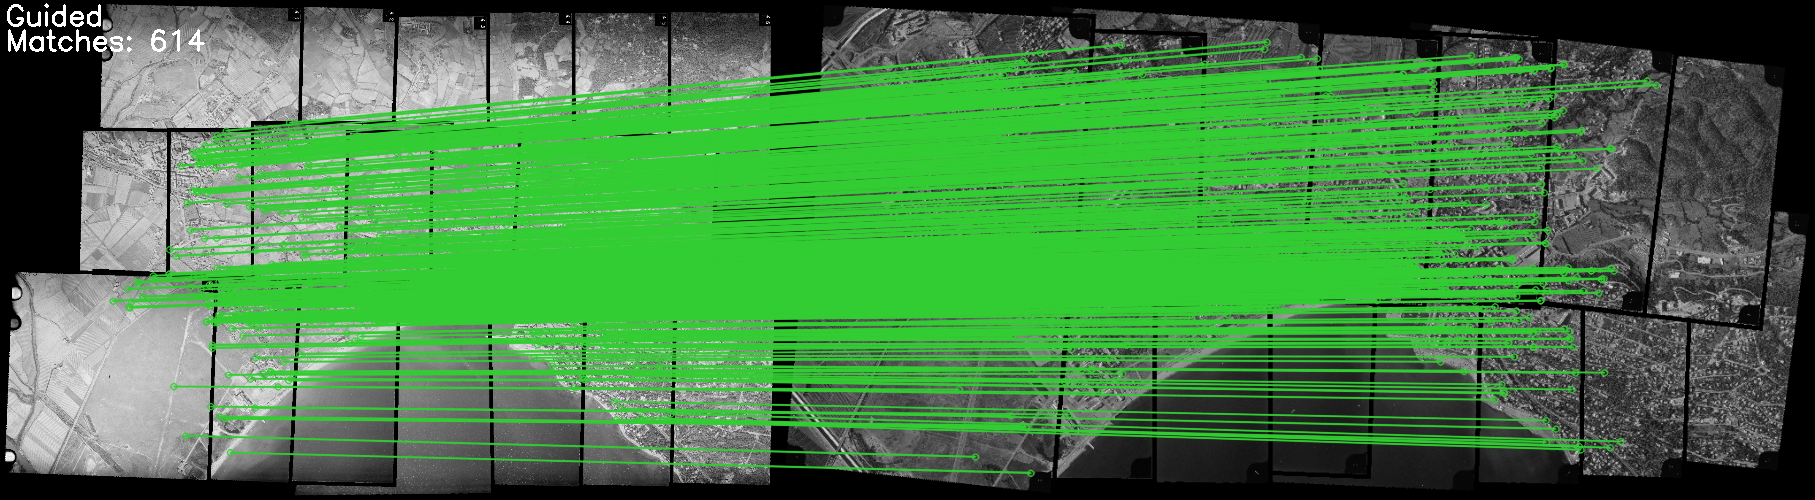
\includegraphics[width=6.8cm]{images/Chapitre4/Precise-SIFTDSMHomol-1954-1966-GuidedSIFT-3DRANSAC-CrossCorrelation-PileImg_Ortho-MEC-Malt_Tapas_1954_Ortho-MEC-Malt_Tapas_1966.png}
			\end{minipage}%
		}
		\caption{Precise matching visualization of \textbf{Fr{\'e}jus 1954 and 1966}. (a) Image pairs to be matched, with red rectangles indicating the overlapping zone. (b) Numbers of tentative, enhanced and final matches recovered with $Patch_{SpGDSM}$, $Guided_{SpGDSM}$, $Patch_{SIFTDSM}$ and $Guided_{SIFTDSM}$ individually. (c-f) Visualization of final matches recovered with $Patch_{SpGDSM}$, $Guided_{SpGDSM}$, $Patch_{SIFTDSM}$ and $Guided_{SIFTDSM}$ individually.}
		\label{MatchVizFrejus1954-1966}
	\end{center}
\end{figure*} 

\begin{figure*}[htbp]
	\begin{center}
		\subfigure[Overlapping zone]{
			\begin{minipage}[t]{0.48\linewidth}
				\centering
				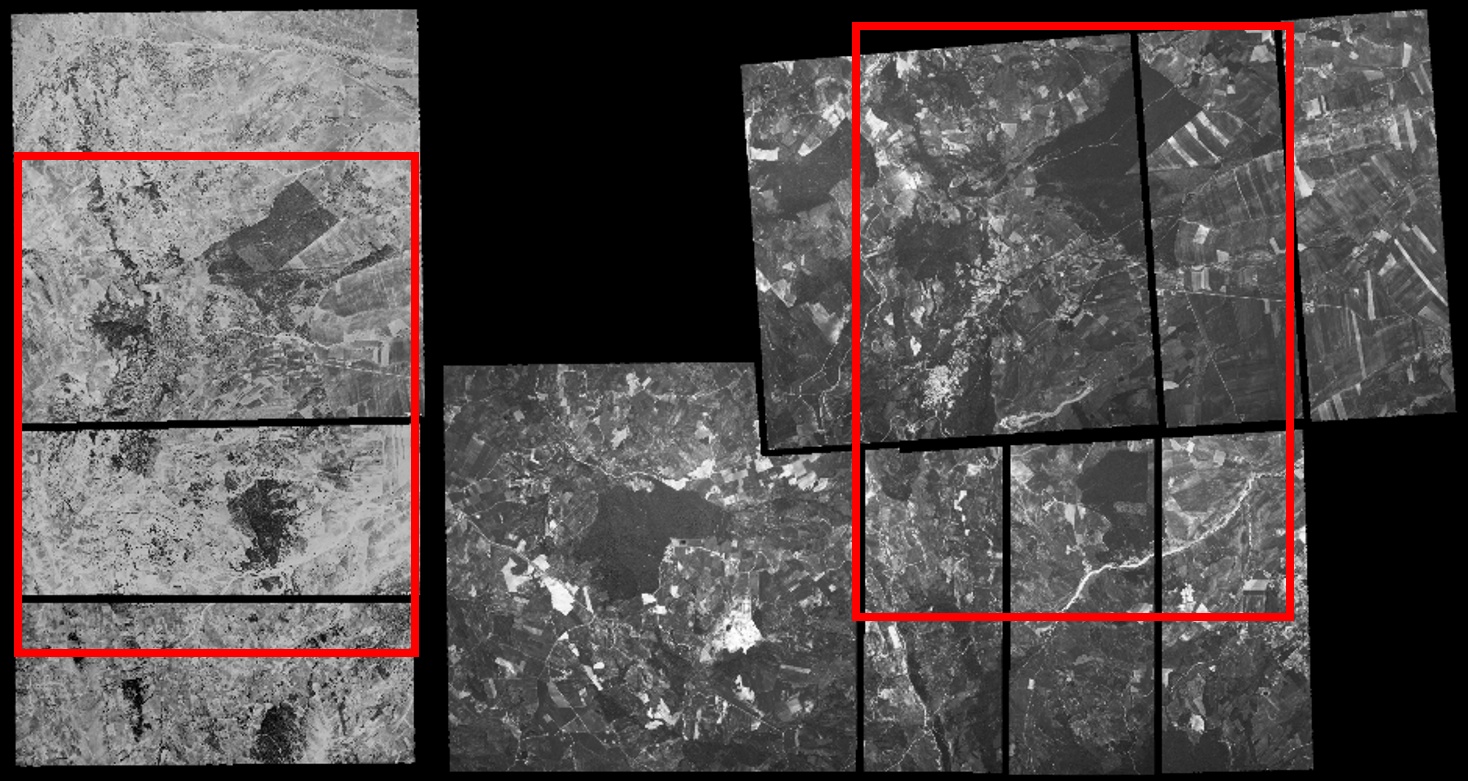
\includegraphics[width=6.8cm]{images/Chapitre3/Pseudo-Ortho-MEC-Malt_Tapas_1954_Ortho-MEC-Malt_Tapas_2003.png}
			\end{minipage}%
		}
		\subfigure[Number of recovered matches]{
			\begin{minipage}[t]{0.48\linewidth}
				\centering
				\includegraphics[width=5.8cm]{images/Chapitre4/PlotBarH-Alberona1954-2003.png}
			\end{minipage}%
		}
		\subfigure[$Patch_{SpGDSM}$]{
			\begin{minipage}[t]{0.48\linewidth}
				\centering
				\includegraphics[width=6.8cm]{images/Chapitre4/Precise-SpGDSMHomol-SuperGlue-3DRANSAC-CrossCorrelation-PileImg_Ortho-MEC-Malt_Tapas_1954_Ortho-MEC-Malt_Tapas_2003.png}
			\end{minipage}%
		}
		\subfigure[$Guided_{SpGDSM}$]{
			\begin{minipage}[t]{0.48\linewidth}
				\centering
				\includegraphics[width=6.8cm]{images/Chapitre4/Precise-SpGDSMHomol-GuidedSIFT-3DRANSAC-CrossCorrelation-PileImg_Ortho-MEC-Malt_Tapas_1954_Ortho-MEC-Malt_Tapas_2003.png}
			\end{minipage}%
		}
		\subfigure[$Patch_{SIFTDSM}$]{
			\begin{minipage}[t]{0.48\linewidth}
				\centering
				\includegraphics[width=6.8cm]{images/Chapitre4/Precise-SIFTDSMHomol-SuperGlue-3DRANSAC-CrossCorrelation-PileImg_Ortho-MEC-Malt_Tapas_1954_Ortho-MEC-Malt_Tapas_2003.png}
			\end{minipage}%
		}
		\subfigure[$Guided_{SIFTDSM}$]{
			\begin{minipage}[t]{0.48\linewidth}
				\centering
				\includegraphics[width=6.8cm]{images/Chapitre4/Precise-SIFTDSMHomol-GuidedSIFT-3DRANSAC-CrossCorrelation-PileImg_Ortho-MEC-Malt_Tapas_1954_Ortho-MEC-Malt_Tapas_2003.png}
			\end{minipage}%
		}
		\caption{Precise matching visualization of \textbf{Alberona 1954 and 2003}. (a) Image pairs to be matched, with red rectangles indicating the overlapping zone. (b) Numbers of tentative, enhanced and final matches recovered with $Patch_{SpGDSM}$, $Guided_{SpGDSM}$, $Patch_{SIFTDSM}$ and $Guided_{SIFTDSM}$ individually. (c-f) Visualization of final matches recovered with $Patch_{SpGDSM}$, $Guided_{SpGDSM}$, $Patch_{SIFTDSM}$ and $Guided_{SIFTDSM}$ individually.}
		\label{MatchVizAlberona}
	\end{center}
\end{figure*} 


%\subsubsection{DoD}
\paragraph{\ac{DoD}.}
%The visualization of \ac{DoD}s for dataset Alberona is demonstrated in~\ref{DoDAlberona}. The corresponding statistical information is displayed in ~\ref{PreciseDoDStatistic}.\\

%As the \ac{DoD}s show similar pattern, for the sake of simplicity, we only show the results of 2 sets of datasets: Fr{\'e}jus and Alberona, as Fr{\'e}jus is interesting for representing the general case for change detection, and Alberona is interesting as it witnessed landslide. For Kobe, the more interesting result is the ground displacement caused by the earthquake, which are demonstrated later, so we move the \ac{DoD}s of Kobe as well as Pezenas to Appendix~\ref{sec:PreciseDoD}.\\

The \ac{DoD}s for Fr{\'e}jus and Alberona are demonstrated in Figure~\ref{PreciseDoDFrejus} and ~\ref{PreciseDoDAlberona}. 
In each figure, the roughly co-registered \ac{DoD}s resulted from rough co-registration variants $SuperGlue_{DSM}$ and $SIFT_{DSM}$ (elaborated in Chapter~\ref{chap:RoughCoReg}, hereinafter referred to as DoD$^{SpGDSM}$ and DoD$^{SIFTDSM}$) are displayed as references, and the refined \ac{DoD}s resulted from variants $Patch_{SpGDSM}$, $Guided_{SpGDSM}$, $Patch_{SIFTDSM}$ and $Guided_{SIFTDSM}$ (hereinafter termed as DoD$^{Patch_{SpGDSM}}$, DoD$^{Guided_{SpGDSM}}$, DoD$^{Patch_{SIFTDSM}}$ and DoD$^{Guided_{SIFTDSM}}$) are given for comparison. 
For the \ac{DoD}s of Alberona, the extent of the landslide area is indicated with black lines based on the landslide inventory map, which is plotted by expert geomorphologists with visual interpretation of aerial photographs. 
The corresponding statistical information is displayed in Table~\ref{PreciseDoDStatistic}.\\


%In conclusion:\\
%\begin{itemize}
%	\item Both precise matching pipelines (i.e., $Patch$ and $Guided$) works, as long as the rough co-registration basic is reliable.\\
%\end{itemize}

%, the \textit{dome} effect presented in DoD$^{SpGDSM}$ and DoD$^{SIFTDSM}$ (the first column of the subgraphs) is effectively mitigated in DoD$^{Patch_{SpGDSM}}$, DoD$^{Guided_{SpGDSM}}$, DoD$^Patch_{SIFTDSM}$ and DoD$^Guided_{SIFTDSM}$ for all the 3 historical epochs (the second and third column of subgraphs), except for (e) \ac{DoD}$_{Frejus1954}^{Patch_{SIFTDSM}}$ and (f) \ac{DoD}$_{Frejus1954}^{Guided_{SIFTDSM}}$. The reason lies in the fact that the rough co-registration basic of (e) and (f) is inferior, as we mentioned in Section ~\ref{sec:matchViz}. For the other \ac{DoD}s resulted from refined orientations, \\
%, thanks to the numerous and accurate matches recovered in the precise matching stage

%Both precise matching pipelines (i.e., $Patch$ and $Guided$) works for all the datasets, as long as the rough co-registration basic is reliable.\\



\begin{figure*}[htbp]
	\begin{center}
		\subfigure[\ac{DoD}$_{Frejus1954}^{{SpGDSM}}$]{
			\begin{minipage}[t]{0.31\linewidth}
				\centering
				\includegraphics[width=3.3cm,trim=740 80 50 230,clip]{images/Chapitre3/DoD1954DSM-SuperGlue.png}
			\end{minipage}%
		}
		\subfigure[\ac{DoD}$_{Frejus1954}^{Patch_{SpGDSM}}$]{
			\begin{minipage}[t]{0.31\linewidth}
				\centering
				\includegraphics[width=3.3cm,trim=740 80 50 230,clip]{images/Chapitre4/DoD1954_Patch_SpGDSM.png}
			\end{minipage}%
		}
		\subfigure[\ac{DoD}$_{Frejus1954}^{Guided_{SpGDSM}}$]{
			\begin{minipage}[t]{0.31\linewidth}
				\centering
				\includegraphics[width=3.3cm,trim=740 80 50 230,clip]{images/Chapitre4/DoD1954_Guided_SpGDSM.png}
			\end{minipage}%
		}\\
		\subfigure[\ac{DoD}$_{Frejus1954}^{{SIFTDSM}}$]{
			\begin{minipage}[t]{0.31\linewidth}
				\centering
				\includegraphics[width=3.3cm,trim=740 100 50 200,clip]{images/Chapitre3/DoD1954DSM-SIFT.png}
			\end{minipage}%
		}
		\subfigure[\ac{DoD}$_{Frejus1954}^{Patch_{SIFTDSM}}$]{
			\begin{minipage}[t]{0.31\linewidth}
				\centering
				\includegraphics[width=3.3cm,trim=740 80 50 230,clip]{images/Chapitre4/DoD1954_Patch_SIFTDSM.png}
			\end{minipage}%
		}
		\subfigure[\ac{DoD}$_{Frejus1954}^{Guided_{SIFTDSM}}$]{
			\begin{minipage}[t]{0.31\linewidth}
				\centering
				\includegraphics[width=3.3cm,trim=740 80 50 230,clip]{images/Chapitre4/DoD1954_Guided_SIFTDSM.png}
			\end{minipage}%
		}\\
		
		\subfigure[\ac{DoD}$_{Frejus1966}^{{SpGDSM}}$]{
			\begin{minipage}[t]{0.31\linewidth}
				\centering
				\includegraphics[width=3.3cm,trim=740 230 50 380,clip]{images/Chapitre3/DoD1966DSM-SuperGlue.png}
			\end{minipage}%
		}
		\subfigure[\ac{DoD}$_{Frejus1966}^{Patch_{SpGDSM}}$]{
			\begin{minipage}[t]{0.31\linewidth}
				\centering
				\includegraphics[width=3.3cm,trim=740 230 50 380,clip]{images/Chapitre4/DoD1966_Patch_SpGDSM.png}
			\end{minipage}%
		}
		\subfigure[\ac{DoD}$_{Frejus1966}^{Guided_{SpGDSM}}$]{
			\begin{minipage}[t]{0.31\linewidth}
				\centering
				\includegraphics[width=3.3cm,trim=740 230 50 380,clip]{images/Chapitre4/DoD1966_Guided_SpGDSM.png}
			\end{minipage}%
		}\\
		\subfigure[\ac{DoD}$_{Frejus1966}^{{SIFTDSM}}$]{
			\begin{minipage}[t]{0.31\linewidth}
				\centering
				\includegraphics[width=3.3cm,trim=740 230 50 380,clip]{images/Chapitre3/DoD1966DSM-SIFT.png}
			\end{minipage}%
		}
		\subfigure[\ac{DoD}$_{Frejus1966}^{Patch_{SIFTDSM}}$]{
			\begin{minipage}[t]{0.31\linewidth}
				\centering
				\includegraphics[width=3.3cm,trim=740 230 50 380,clip]{images/Chapitre4/DoD1966_Patch_SIFTDSM.png}
			\end{minipage}%
		}
		\subfigure[\ac{DoD}$_{Frejus1966}^{Guided_{SIFTDSM}}$]{
			\begin{minipage}[t]{0.31\linewidth}
				\centering
				\includegraphics[width=3.3cm,trim=740 230 50 380,clip]{images/Chapitre4/DoD1966_Guided_SIFTDSM.png}
			\end{minipage}%
		}\\
		
		
		\subfigure[\ac{DoD}$_{Frejus1970}^{{SpGDSM}}$]{
			\begin{minipage}[t]{0.31\linewidth}
				\centering
				\includegraphics[width=3.3cm,trim=680 180 50 260,clip]{images/Chapitre3/DoD1970DSM-SuperGlue.png}				
			\end{minipage}%
		}
		\subfigure[\ac{DoD}$_{Frejus1970}^{Patch_{SpGDSM}}$]{
			\begin{minipage}[t]{0.31\linewidth}
				\centering
				\includegraphics[width=3.3cm,trim=700 180 50 260,clip]{images/Chapitre4/DoD1970_Patch_SpGDSM.png}
			\end{minipage}%
		}
		\subfigure[\ac{DoD}$_{Frejus1970}^{Guided_{SpGDSM}}$]{
			\begin{minipage}[t]{0.31\linewidth}
				\centering
				\includegraphics[width=3.3cm,trim=700 180 50 260,clip]{images/Chapitre4/DoD1970_Guided_SpGDSM.png}
			\end{minipage}%
		}\\
		\subfigure[\ac{DoD}$_{Frejus1970}^{{SIFTDSM}}$]{
			\begin{minipage}[t]{0.31\linewidth}
				\centering
				\includegraphics[width=3.3cm,trim=680 180 50 260,clip]{images/Chapitre3/DoD1970DSM-SIFT.png}
			\end{minipage}%
		}
		\subfigure[\ac{DoD}$_{Frejus1970}^{Patch_{SIFTDSM}}$]{
			\begin{minipage}[t]{0.31\linewidth}
				\centering
				\includegraphics[width=3.3cm,trim=700 180 50 260,clip]{images/Chapitre4/DoD1970_Patch_SIFTDSM.png}
			\end{minipage}%
		}
		\subfigure[\ac{DoD}$_{Frejus1970}^{Guided_{SIFTDSM}}$]{
			\begin{minipage}[t]{0.31\linewidth}
				\centering
				\includegraphics[width=3.3cm,trim=700 180 50 260,clip]{images/Chapitre4/DoD1970_Guided_SIFTDSM.png}
			\end{minipage}%
		}\\
		
		\subfigure[\ac{DoD} legend]{
			\begin{minipage}[t]{1\linewidth}
				\centering
				\includegraphics[width=11cm]{images/Chapitre4/LegendDoD.png}
			\end{minipage}%
		}
		\caption{(a-f) \ac{DoD}s between free epoch \textbf{Fr{\'e}jus 1954} and reference epoch \textbf{2014}. (g-l) \ac{DoD}s between free epoch \textbf{Fr{\'e}jus 1966} and reference epoch \textbf{2014}. (m-r) \ac{DoD}s between free epoch \textbf{Fr{\'e}jus 1970} and reference epoch \textbf{2014}. (a, d, g, j, m, p) are roughly co-registered \ac{DoD}s resulted from variants $SuperGlue_{DSM}$ and $SIFT_{DSM}$ (elaborated in Chapter \ref{chap:RoughCoReg}). (b, c, e, f, h, i, k, l, n, o, q, r) are refined \ac{DoD}s resulted from variants $Patch_{SpGDSM}$, $Guided_{SpGDSM}$, $Patch_{SIFTDSM}$ and $Guided_{SIFTDSM}$ individually.}
		\label{PreciseDoDFrejus}
	\end{center}
\end{figure*} 


\begin{figure*}[htbp]
	\begin{center}
		\subfigure[\ac{DoD}$_{Alberona}^{{SpGDSM}}$]{
			\begin{minipage}[t]{0.31\linewidth}
				\centering
				%\includegraphics[width=4.3cm,trim=870 100 180 180,clip]{images/Chapitre3/DoDAlberona1954DSM-SuperGlue.png}
				\includegraphics[width=4.5cm,trim=605 35 440 160,clip]{images/Chapitre4/AlberonaDoD1954_SpGDSM.png}
			\end{minipage}%
		}
		\subfigure[\ac{DoD}$_{Alberona}^{Patch_{SpGDSM}}$]{
			\begin{minipage}[t]{0.31\linewidth}
				\centering
				\includegraphics[width=4.6cm,trim=580 30 780 160,clip]{images/Chapitre4/AlberonaDoD1954_Patch_SpGDSM.png}
			\end{minipage}%
		}
		\subfigure[\ac{DoD}$_{Alberona}^{Guided_{SpGDSM}}$]{
			\begin{minipage}[t]{0.31\linewidth}
				\centering
				\includegraphics[width=4.5cm,trim=560 30 810 160,clip]{images/Chapitre4/AlberonaDoD1954_Guided_SpGDSM.png}
			\end{minipage}%
		}\\
		\subfigure[\ac{DoD}$_{Alberona}^{{SIFTDSM}}$]{
			\begin{minipage}[t]{0.31\linewidth}
				\centering
				%\includegraphics[width=4.3cm,trim=870 100 180 180,clip]{images/Chapitre3/DoDAlberona1954DSM-SIFT.png}
				\includegraphics[width=4.5cm,trim=605 35 440 160,clip]{images/Chapitre4/AlberonaDoD1954_SIFTDSM.png}
			\end{minipage}%
		}
		\subfigure[\ac{DoD}$_{Alberona}^{Patch_{SIFTDSM}}$]{
			\begin{minipage}[t]{0.31\linewidth}
				\centering
				\includegraphics[width=4.6cm,trim=580 30 780 160,clip]{images/Chapitre4/AlberonaDoD1954_Patch_SIFTDSM.png}
			\end{minipage}%
		}
		\subfigure[\ac{DoD}$_{Alberona}^{Guided_{SIFTDSM}}$]{
			\begin{minipage}[t]{0.31\linewidth}
				\centering
				\includegraphics[width=4.5cm,trim=560 30 810 160,clip]{images/Chapitre4/AlberonaDoD1954_Guided_SIFTDSM.png}
			\end{minipage}%
		}
		
		\subfigure[\ac{DoD} legend]{
			\begin{minipage}[t]{1\linewidth}
				\centering
				\includegraphics[width=11cm]{images/Chapitre4/LegendDoD.png}
			\end{minipage}%
		}
		\caption{\ac{DoD}s between free epoch \textbf{Alberona 1954} and reference epoch \textbf{2003}. (a) and (d) are roughly co-registered \ac{DoD}s resulted from variants $SuperGlue_{DSM}$ and $SIFT_{DSM}$ (elaborated in Chapter \ref{chap:RoughCoReg}). (b, c, e, f) are refined \ac{DoD}s resulted from variants $Patch_{SpGDSM}$, $Guided_{SpGDSM}$, $Patch_{SIFTDSM}$ and $Guided_{SIFTDSM}$ individually.}
		\label{PreciseDoDAlberona}
	\end{center}
\end{figure*} 


%
%\begin{table}%[H]
%	\footnotesize
%	\centering
%	\begin{tabular}{||l|l|c|c|c||}\hline
%		& &$\mu$ [m]&$\sigma$ [m]&$|\mu|$ [m]\\\hline\hline
%%		\multirow{6}{*}{$DoD^{Frejus}_{1954-2014}$}
%%		&${SuperGlue_{ImgPairs}}$ & 5.70 & 6.32 & 6.62\\
%%		&${SuperGlue_{Ortho}}$ & 2.19 & 6.46 & 4.55\\
%%		&${SuperGlue_{DSM}}$ & 2.07 & 4.87 & \textbf{3.83} \\
%%		&${SIFT_{ImgPairs}}$ & / & / & / \\
%%		&${SIFT_{Ortho}}$ & / & / & / \\
%%		&${SIFT_{DSM}}$ & 6.92 & 8.47 & 8.04\\\hline
%%		
%%		\multirow{6}{*}{$DoD^{Frejus}_{1966-2014}$}
%%		&${SuperGlue_{ImgPairs}}$ & -1.36 & 3.82 & 2.90\\
%%		&${SuperGlue_{Ortho}}$ & -0.37 & 4.22 & 3.01\\
%%		&${SuperGlue_{DSM}}$ & -0.46 & 3.77 & \textbf{2.68}\\
%%		&${SIFT_{ImgPairs}}$ & / & / & / \\
%%		&${SIFT_{Ortho}}$ & / & / & / \\
%%		&${SIFT_{DSM}}$ & -1.72 & 4.92 & 3.75\\\hline
%%		
%%		\multirow{6}{*}{$DoD^{Frejus}_{1970-2014}$}
%%		&${SuperGlue_{ImgPairs}}$ & -5.04 & 5.09 & 5.70\\
%%		&${SuperGlue_{Ortho}}$ & -2.63 & 5.18 & \textbf{4.39}\\
%%		&${SuperGlue_{DSM}}$ & -1.71 & 5.75 & 4.61\\
%%		&${SIFT_{ImgPairs}}$ & / & / & / \\
%%		&${SIFT_{Ortho}}$ & / & / & / \\
%%		&${SIFT_{DSM}}$ & -3.17 & 5.44 & 4.71\\\hline
%		
%		%%%%%%%%%%%%%%%%%%%%%%%%satellite
%		\multirow{4}{*}{$DoD^{Pezenas}_{1971-2014(Satellite)}$}
%&${Patch_{SpGDSM}}$ & -0.34 & 4.39 & 2.28\\
%&${Guided_{SpGDSM}}$ & -0.65 & 4.46 & 2.45\\
%&${Patch_{SIFTDSM}}$ & -0.49 & 4.41 & 2.29\\
%&${Guided_{SIFTDSM}}$ & -0.57 & 4.38 & \textbf{2.27}\\\hline
%
%
%%		\multirow{4}{*}{$DoD^{Pezenas}_{1971-2014(Satellite)}$}
%%		%&${SuperGlue_{DSM}}$ & -3.70 & 10.65 & 8.29\\
%%		&${Patch_{SpGDSM}}$ & -0.45 & 4.62 & 2.34\\
%%		&${Guided_{SpGDSM}}$ & -0.61 & 4.75 & 2.47\\
%%		%&${SIFT_{DSM}}$ & -0.68 & 8.11 & 5.80 \\
%%		&${Patch_{SIFTDSM}}$ & -0.35 & 4.70 & \textbf{2.28}\\
%%		&${Guided_{SIFTDSM}}$ & -0.48 & 4.39 & 2.33\\\hline
%				
%%		&${SuperGlue_{Ortho}}$ & / & / & /\\
%%		&${SuperGlue_{DSM}}$ & -3.70 & 10.65 & 8.29\\
%%		%&${SuperGlue_{DSM}}$ & -1.85 & 13.24 & 9.15\\
%%		&${SIFT_{Ortho}}$ & / & / & /\\
%%		&${SIFT_{DSM}}$ & -0.68 & 8.11 & \textbf{5.80} \\\hline
%%		%&${SIFT_{DSM}}$ & 0.58 & 7.82 & \textbf{3.18}\\\hline
%		
%		\multirow{6}{*}{$DoD^{Kobe}_{1991-1995}$}
%		&${Patch_{SpGDSM}}$ & 1.93 & 10.26 & 3.99\\
%		&${Guided_{SpGDSM}}$ & 2.03 & 11.74 & 4.30\\
%		&${Patch_{SIFTDSM}}$ & 1.80 & 10.36 & 4.00\\
%		&${Guided_{SIFTDSM}}$ & 1.84 & 9.48 & \textbf{3.87}\\
%
%%		&${SuperGlue_{ImgPairs}}$ & -1.63 & 13.85 & \textbf{7.24}\\
%%		%&${SIFT_{ImgPairs}}$ & 167.46 & 121.26 & 168.47\\
%%		&${SuperGlue_{Ortho}}$ & -0.54 & 14.83 & 7.78\\
%%		%&${SIFT_{Ortho}}$ & 4.29 & 41.89 & 26.01\\
%%		&${SuperGlue_{DSM}}$ & -0.75 & 14.62 & 7.95\\
%%		&${SIFT_{ImgPairs}}$ & / & / & / \\
%%		&${SIFT_{Ortho}}$ & / & / & / \\
%%		&${SIFT_{DSM}}$ & 0.27 & 14.40 & 7.57\\\hline
%		
%	\end{tabular}
%	\caption{Average value $\mu$, standard deviation $\sigma$, and absolute average value $|\mu|$ of all the \ac{DoD}s in Figure~\ref{DoDFrejus}, ~\ref{DoDPezenas}, ~\ref{DoDPezenas-Satellite} and ~\ref{DoDKobe}.}
%	\label{PreciseDoDStatistic}
%\end{table}


\begin{table}%[H]
	\footnotesize
	\centering
	\begin{tabular}{||l|l|c|c|c||}\hline
		& &$\mu$ [m]&$\sigma$ [m]&$|\mu|$ [m]\\\hline\hline
\multirow{6}{*}{$DoD^{Frejus}_{1954-2014}$}
&${SpGDSM}$ & 2.24 & 5.34 & {4.35}\\
&${Patch_{SpGDSM}}$ & -1.89 & 4.16 & 2.93\\
&${Guided_{SpGDSM}}$ & -1.29 & 4.03 & \textbf{2.65}\\
&${SIFTDSM}$ & 6.91 & 8.90 & 8.45\\
&${Patch_{SIFTDSM}}$ & -6.17 & 6.54 & 6.69\\
&${Guided_{SIFTDSM}}$ & 3.72 & 17.12 & 12.90\\\hline

\multirow{6}{*}{$DoD^{Frejus}_{1966-2014}$}
&${SpGDSM}$ & -0.80 & 4.71 & {3.28}\\
&${Patch_{SpGDSM}}$ & -0.93 & 4.00 & 2.57\\
&${Guided_{SpGDSM}}$ & -0.51 & 3.93 & \textbf{2.45}\\
&${SIFTDSM}$ & -2.12 & 5.66 & 4.42\\
&${Patch_{SIFTDSM}}$ & -0.99 & 4.01 & 2.58\\
&${Guided_{SIFTDSM}}$ & -0.24 & 3.92 & 2.56\\\hline


\multirow{6}{*}{$DoD^{Frejus}_{1970-2014}$}
&${SpGDSM}$ & -2.37 & 6.57 & {5.35}\\
&${Patch_{SpGDSM}}$ & -1.18 & 3.83 & 2.38\\
&${Guided_{SpGDSM}}$ & -0.46 & 3.83 & \textbf{2.37}\\
&${SIFTDSM}$ & -3.76 & 6.21 & 5.47\\
&${Patch_{SIFTDSM}}$ & -1.28 & 3.92 & 2.45\\
&${Guided_{SIFTDSM}}$ & -0.43 & 3.79 & 2.40\\\hline

%&${{SpGDSM}}$ & 2.07 & 4.87 & {3.83} \\
%&${Patch_{SpGDSM}}$ & -1.91 & 3.24 & 2.69\\
%&${Guided_{SpGDSM}}$ & -1.33 & 3.28 & \textbf{2.30}\\
%&${{SIFTDSM}}$ & 6.92 & 8.47 & 8.04\\
%&${Patch_{SIFTDSM}}$ & -6.28 & 6.72 & 6.62\\
%&${Guided_{SIFTDSM}}$ & 3.58 & 16.62 & 12.56\\\hline
%
%\multirow{6}{*}{$DoD^{Frejus}_{1966-2014}$}
%&${{SpGDSM}}$ & -0.46 & 3.77 & {2.68}\\
%&${Patch_{SpGDSM}}$ & -0.56 & 3.44 & 2.27\\
%&${Guided_{SpGDSM}}$ & -0.12 & 3.45 & \textbf{2.19}\\
%&${{SIFTDSM}}$ & -1.72 & 4.92 & 3.75\\
%&${Patch_{SIFTDSM}}$ & -0.59 & 3.36 & 2.29\\
%&${Guided_{SIFTDSM}}$ & 0.14 & 3.35 & 2.25\\\hline
%
%\multirow{6}{*}{$DoD^{Frejus}_{1970-2014}$}
%&${{SpGDSM}}$ & -1.71 & 5.75 & 4.61\\
%&${Patch_{SpGDSM}}$ & -0.86 & 3.20 & 2.12\\
%&${Guided_{SpGDSM}}$ & -0.18 & 3.27 & 2.12\\
%&${{SIFTDSM}}$ & -3.17 & 5.44 & 4.71\\
%&${Patch_{SIFTDSM}}$ & -0.98 & 3.26 & 2.20\\
%&${Guided_{SIFTDSM}}$ & -0.15 & 3.17 & \textbf{2.05}\\\hline		

\multirow{6}{*}{$DoD^{Alberona}_{1954-2003}$}
&${SpGDSM}$ & -0.28 & 7.84 & 6.17\\
&${Patch_{SpGDSM}}$ & -0.80 & 4.44 & 3.22\\
&${Guided_{SpGDSM}}$ & -0.20 & 6.20 & 4.86\\
&${SIFTDSM}$ & -1.88 & 7.44 & 5.89\\
&${Patch_{SIFTDSM}}$ & -1.00 & 3.73 & \textbf{2.75}\\
&${Guided_{SIFTDSM}}$ & 2.11 & 5.86 & 4.63\\\hline
	\end{tabular}
	\caption{Average value $\mu$, standard deviation $\sigma$, and absolute average value $|\mu|$ of all the \ac{DoD}s in Figure~\ref{PreciseDoDFrejus} and ~\ref{PreciseDoDAlberona}.}
	\label{PreciseDoDStatistic}
\end{table}


%\subsubsection{Ground displacement}
\paragraph{Ground displacement (i.e., Gd).}
The northeastward Gd %ground displacement %(hereinafter termed as Gd)
maps of Kobe dataset as well as the ground truth Gd provided by the Japan meteorological agency~\cite{ian1996morphological} are presented in Figure~\ref{GdKobe}. 
The roughly co-registered Gds resulted from variants $SuperGlue_{DSM}$ and $SIFT_{DSM}$ (i.e., Figure~\ref{GdKobe} (b) and (e), elaborated in Chapter~\ref{chap:RoughCoReg}) are displayed as references, and the refined Gds resulted from variants $Patch_{SpGDSM}$, $Guided_{SpGDSM}$, $Patch_{SIFTDSM}$ and $Guided_{SIFTDSM}$ (i.e., Figure~\ref{GdKobe} (c, d) and (f, g)) are given for comparison. 

\begin{figure*}[htbp]
	\begin{center}
		\subfigure[Gd$_{Kobe}^{{GT}}$]{
			\begin{minipage}[t]{1\linewidth}
				\centering
				\includegraphics[width=9cm]{images/Chapitre4/Kobe-faultmap.png}
			\end{minipage}%
		}
		\subfigure[Gd$_{Kobe}^{{SpGDSM}}$]{
			\begin{minipage}[t]{1\linewidth}
				\centering
				\includegraphics[width=9cm,trim=680 330 100 570,clip]{images/Chapitre4/Gd1991_SpGDSM.png}
			\end{minipage}%
		}
		\subfigure[Gd$_{Kobe}^{Patch_{SpGDSM}}$]{
			\begin{minipage}[t]{1\linewidth}
				\centering
				\includegraphics[width=9cm,trim=680 330 100 570,clip]{images/Chapitre4/Gd1991_Patch_SpGDSM.png}
			\end{minipage}%
		}
		\subfigure[Gd$_{Kobe}^{Guided_{SpGDSM}}$]{
			\begin{minipage}[t]{1\linewidth}
				\centering
				\includegraphics[width=9cm,trim=680 330 100 570,clip]{images/Chapitre4/Gd1991_Guided_SpGDSM.png}
			\end{minipage}%
		}\\
		\subfigure[Gd$_{Kobe}^{{SIFTDSM}}$]{
			\begin{minipage}[t]{1\linewidth}
				\centering
				\includegraphics[width=9cm,trim=680 330 100 570,clip]{images/Chapitre4/Gd1991_SIFTDSM.png}
			\end{minipage}%
		}
		\subfigure[Gd$_{Kobe}^{Patch_{SIFTDSM}}$]{
			\begin{minipage}[t]{1\linewidth}
				\centering
				\includegraphics[width=9cm,trim=680 330 100 570,clip]{images/Chapitre4/Gd1991_Patch_SIFTDSM.png}
			\end{minipage}%
		}
		\subfigure[Gd$_{Kobe}^{Guided_{SIFTDSM}}$]{
			\begin{minipage}[t]{1\linewidth}
				\centering
				\includegraphics[width=9cm,trim=680 330 100 570,clip]{images/Chapitre4/Gd1991_Guided_SIFTDSM.png}
			\end{minipage}%
		}
		
		\subfigure[Gd legend]{
			\begin{minipage}[t]{1\linewidth}
				\centering
				\includegraphics[width=11cm]{images/Chapitre4/legend-Gd.png}
			\end{minipage}%
		}
		\caption{ground displacement(Gd) between free epoch \textbf{Kobe 1991} and reference epoch \textbf{1995}. (a) is the ground truth Gd provided by the Japan meteorological agency. (b) and (e) are roughly co-registered Gds resulted from variants $SuperGlue_{DSM}$ and $SIFT_{DSM}$ (elaborated in Chapter \ref{chap:RoughCoReg}). (c, d, f, g) are refined Gds resulted from variants $Patch_{SpGDSM}$, $Guided_{SpGDSM}$, $Patch_{SIFTDSM}$ and $Guided_{SIFTDSM}$ individually.}
		\label{GdKobe}
	\end{center}
\end{figure*} 

\paragraph{Discussion.}
\label{para:DiscussionP}
As can be seen, both $Patch$ and $Guided$ recover a lot of matches, except for the ones involving epoch 1954 based on rough co-registration of $SIFT_{DSM}$ (Figure \ref{MatchVizFrejus1954-2014} (e, f), \ref{MatchVizFrejus1954-1970} (e, f) and \ref{MatchVizFrejus1954-1966} (e, f)). It is because the rough co-registration result of $SIFT_{DSM}$ for epoch 1954 is unsatisfactory, as was mentioned in Section ~\ref{sec:MatchVizMainBody}.
%As the basics of rough co-registration are reliable, both $Patch$ and $Guided$ recovered a lot of final matches for all the variants.
Besides, 3D-RANSAC filter and cross correlation removed a considerable number of matches, at the same time enough matches survived, which guaranteed robustness of our method. %Moreover, $Patch$ recovered more matches than $Guided$, which is understandable as SuperGlue is more invariant over time than SIFT.\\
\par
%Similar pattern appears for the datasets Pezenas and Kobe. For more details please refer to Appendix~\ref{sec:PrecisematchViz}.
For the \ac{DoD}s, the \textit{dome} effect appears in all the DoD$^{SpGDSM}$ and DoD$^{SIFTDSM}$ (i.e., the first column of the subgraphs in Figure~\ref{PreciseDoDFrejus} and \ref{PreciseDoDAlberona}), as the camera parameters are poorly estimated without the precise matches.\\
%For the other \ac{DoD}s resulted from orientations refined with our precise matches (i.e., the second and third columns of subgraphs in Figure~\ref{PreciseDoDFrejus} and \ref{PreciseDoDAlberona}), 
For most refined \ac{DoD}s in Fr{\'e}jus (i.e., the second and third columns of subgraphs in Figure~\ref{PreciseDoDFrejus} except for (e) and (f)), the \textit{dome} effect is effectively mitigated, thanks to our numerous and precise matches. In the meantime, the real scene changes are preserved, such as the new buildings and seaports.\\
For Figure~\ref{PreciseDoDFrejus} (e) \ac{DoD}$_{Frejus1954}^{Patch_{SIFTDSM}}$ and (f) \ac{DoD}$_{Frejus1954}^{Guided_{SIFTDSM}}$, the \textit{dome} effect is even worse than the roughly co-registered one (i.e., Figure~\ref{PreciseDoDFrejus} (d) \ac{DoD}$_{Frejus1954}^{{SIFTDSM}}$) due to low quality of matches shown in Figure \ref{MatchVizFrejus1954-2014} (e, f), \ref{MatchVizFrejus1954-1970} (e, f) and \ref{MatchVizFrejus1954-1966} (e, f).\\
For the refined \ac{DoD}s in Alberona, the \textit{dome} effect is mitigated for the variant $Patch$, but not for $Guided$, as the images from different epochs showed various tone, which is challenging for $Guided$. Besides, the images are poorly preserved and scanned with non photogrammetric scanner, and limited number of images leads to a lack of redundant observation. Therefore, only the \ac{DoD}$_{Alberona}^{Patch_{SIFTDSM}}$ (i.e., Figure~\ref{PreciseDoDAlberona} (e)) showed both useful signs in the landslide zone and limited systematic errors in the whole block, as it is based on good matches recovered with $Patch$ variant under the good rough co-registration resulted from $SIFT_{DSM}$.\\
%According to the absolute average value $|\mu|$ of all the \ac{DoD}s in Figure~\ref{PreciseDoDFrejus} and ~\ref{PreciseDoDAlberona} (cf. Talbe \ref{PreciseDoDStatistic}), $Guided$ leads to \ac{DoD}s with slightly better accuracy, even though it is less invariant than $Patch$, it recovers less numerous but more precise matches with the help of rough co-registered orientations and \ac{DSM}s.
\par
For the Gds, an up-lateral strike-slip movement along the sea is present in Figure~\ref{GdKobe} (c, d) and (f, g), but not in (b) and (e). The observed signal is coherent with the fault of the Kobe earthquake known from \ac{GT} (i.e., Figure~\ref{GdKobe} (a)), according to which a striking north $30^{\circ}$-$60^{\circ}$ east rupture occurred along the northeast-southwest coastline across $ \sim $18 km.\\


\section{Conclusion}
In this section we elaborate two variants for precise matching: $Patch$ and $Guided$. 
We test each variant based on two sets of rough co-registration results: $SIFT_{DSM}$ and $SuperGlue_{DSM}$, which leads to 4 variants (i.e., \ding{172} $Patch_{SpGDSM}$, \ding{173} $Guided_{SpGDSM}$, \ding{174} $Patch_{SIFTDSM}$ and \ding{175} $Guided_{SIFTDSM}$.
Experiments are performed on 4 sets of datasets (Fr{\'e}jus, Pezenas, Kobe and Alberona), including the cases of (1) matching aerial epochs only and (2) matching aerial and satellite epochs mixed.
Experiments show that:\\
\begin{enumerate}
	\item Both precise matching variants (i.e., $Patch$ and $Guided$) are capable of recovering numerous and accurate matches, as long as the rough co-registration result is reliable.\\
	\item By adopting the precise matches in a \ac{BBA} routine, the systematic errors in the surfaces can be effectively mitigated while the real scene changes stay.
\end{enumerate}
%Our pipelines are able to provide precise results for variable application cases including general change detection, landslides and earthquakes.


